
% --- Paquetes ---

% Básicos
\documentclass[letterpaper]{article}
\usepackage[english, spanish, mexico, es-noitemize]{babel}
\usepackage{float}
% Matemáticas avanzadas
\usepackage[tbtags]{amsmath}
\usepackage{amssymb, amsthm, mathtools, physics}
\usepackage{tabularx}
\usepackage[nolimits]{cmupint}% Integrales rectas
%\usepackage{siunitx}% Unidades del SI

% Selección de fuente: Descomente el segundo bloque y comente el primero para cambiar entre las dos fuentes

% Latin Modern, fuente estándar
\usepackage{lmodern}
\usepackage[T1]{fontenc}

% TeX Gyre Schola con fouriernc para mates consistentes con la fuente
%\usepackage{fouriernc}
%\usepackage[scale=0.92]{tgschola}
%\usepackage[T1]{fontenc}

% Configuración del documento
\usepackage[margin=1in, top=1.25in, headheight=2\baselineskip, headsep=\baselineskip]{geometry}
\usepackage{fancyhdr}
\usepackage[pdfusetitle, colorlinks]{hyperref}
\usepackage[shortlabels, inline]{enumitem}
\usepackage{multicol, array}
\usepackage{titlesec}
\usepackage[titles]{tocloft}
\usepackage{xcolor, xpatch, calc}

% Gráficos
\usepackage{graphicx, booktabs, wrapfig, pdfpages}
\usepackage{pgfplots}
\usepackage[framemethod=tikz]{mdframed}
\usepackage[outline]{contour}
\usepackage[hang, labelfont=bf, labelsep=period, margin=0.5in]{caption}
\usepackage{subcaption}

% Bibliografía
\usepackage[backend=biber]{biblatex}
\usepackage{csquotes}
\addbibresource{repbib.bib}

% Texto de prueba
\usepackage{lipsum}

% --- Información del documento ---

\title{\mytitle}
\author{\myauthor}
\date{\thedate}

\newcommand{\mytitle}%
	{Proyecto de investigación II:}
	
\newcommand{\mysubtitle}%
	{Revisión sistemática de: Visión computacional para la identificación de objetos en la movilidad de personas con discapacidad visual}

\newcommand{\myauthor}%
	{Estefany Paola Mamani Gutierrez}

\newcommand{\myemail}%
	{\href{mailto:estefanyp.magu@gmail.com}%
	{\texttt{estefanyp.magu@gmail.com}}}%

\newcommand{\thedate}%
	{\today}

\newcommand{\thesubject}%
	{E. P. Ingeniería de Sistemas e Informática}

\newcommand{\firstinstitute}%
	{Facultad de Ingeniería y Arquitectura}

\newcommand{\secondinstitute}%
	{Universidad Nacional de Moquegua}

\newcommand{\shortinstitute}%
	{Facultad de Ingeniería y Arquitectura}

% --- Configuraciones adicionales ---

% Idioma en el preámbulo
\selectspanish

% Librerías de pgfplots
\usepgfplotslibrary{colormaps}

% Librerías de tikz
\usetikzlibrary{babel, calc, scopes, intersections, angles, quotes, arrows, arrows.meta, backgrounds, shapes.geometric, patterns, shadows, perspective, external}

% Descomentar la siguiente línea para externalizar gráficos
%\tikzexternalize

% Versión de PGFplots
\pgfplotsset{compat=newest}

% Definición de estilos de Tikz, etc.
\tikzset{%
	% Configuraciones de tikz particulares del documento, como estilos de nodos y dibujos
	font = {\selectfont},
	frame/.style={thin, dashed, lightgray, line cap=round, rounded corners=5pt}
}

% Grosor de contorno adicional (para emplearse en gráficos)
\contourlength{1pt}

% Directorios de gráficos
\graphicspath{{imágenes/}{escudos/}}

% Todos los enlaces del documento en negro
\hypersetup{allcolors=black}

% Listas personalizadas
\setlist[enumerate, 1]{%
	label=\textbf{\color{\emphcolor}\arabic*.},
	labelindent=\parindent,
	itemindent=*,
	ref=\textbf{\arabic*}
}
\setlist[enumerate, 2]{%
	label=\textbf{\color{\emphcolor}(\alph*)},
	itemindent=*,
	ref=\textbf{(\alph*)}
}
\setlist[enumerate, 3]{%
	label=\color{\emphcolor}\roman*.,
	itemindent=*,
	ref=\roman*
}

% Redefinición de "y otros" en la bibliografía
\DefineBibliographyStrings{spanish}{andothers={et~al\adddot}}

% Personalización de ToC
\renewcommand{\cftdotsep}{1}
\renewcommand{\cftsecleader}{\cftdotfill{\cftdotsep}}
\renewcommand{\cftsecpresnum}{\color{\emphcolor}}
\renewcommand{\cftsecaftersnum}{.}
\setlength{\cftsecindent}{25pt}
\renewcommand{\cftsecafterpnum}{\hspace*{25pt}}
\setlength{\cftbeforesecskip}{\baselineskip/2}

% --- Comandos de mate adicionales ---

\newcommand{\rtwovec}[2]{% Vectores columna en R^2 
	\begin{bmatrix*}[r]
		#1 \\ #2 
	\end{bmatrix*}
}

\newcommand{\rthreevec}[3]{% Vectores columna en R^3
	\begin{bmatrix*}[r]
		#1 \\ #2 \\ #3
	\end{bmatrix*}
}

\newcommand{\uvec}[1]{% Vectores unitarios (con gorrito)
	\textbf{\^{#1}}
}

\newenvironment{amatrix}[2]{% Matices aumentadas
	\left[\begin{array}{@{}*{#1}{r}|*{#2}{r}@{}}
	}%
	{
	\end{array}\right]
}

\DeclareMathOperator{\mcd}{mcd}% Máximo común divisor
\DeclareMathOperator{\midd}{med}% Número medio

% Descomentar esta línea si se elige fouriernc para la fuente matemática y emplear en vez de \nabla
%\newcommand{\Nabla}{\scalebox{1.075}{$\nabla$}}

% --- Diseño de documento ---

% Colores
% \definecolor{emphcolor}{HTML}{0B4166}% Color de énfasis personalizado
\newcommand{\emphcolor}{gray}% Escribir emphcolor dentro de las llaves, si se define

% Longitudes
%\setlength{\columnsep}{0.5in}% Separación entre columnas

% Diseño de títulos de sección
\titleformat{\section}[hang]
{\Large\centering\bfseries}
{\thetitle.}{\widthof{\ }}{\Large\color{\emphcolor}}

% Título de documento
\newcommand{\cover}{%
	\thispagestyle{plain}
	\begin{center}
		\Large\textbf{\textcolor{\emphcolor}{\mytitle}} \\
		\LARGE\textbf{\mysubtitle}
		\bigskip
		
		\normalsize\myauthor \\
		\small\myemail
		\medskip
		
		\normalsize\firstinstitute \\ 
		\secondinstitute
		\medskip
		
		\normalsize\thedate \\
	\end{center}%
}

% Comandos para ingresar keywords en el abstract
\newcommand{\espkeywords}{\noindent\textit{Palabras clave:\ }}
\newcommand{\engkeywords}{\noindent\textit{Keywords:\ }}

% Tipos de columna útiles
\newcolumntype{P}[1]{>{\centering\arraybackslash}p{#1}}
\newcolumntype{M}[1]{>{\centering\arraybackslash}m{#1}}
\newcolumntype{R}[1]{>{\arraybackslash}m{#1}}

% Rediseño del estilo plain
\fancypagestyle{plain}{%
	\renewcommand{\headrulewidth}{0pt}
	
	\fancyhf{}
	\fancyfoot[c]{%
		\begin{tabular}{M{1em}@{}M{2em}@{}M{1em}}
			\textcolor{\emphcolor}{$\boldsymbol{-}$}
			& \thepage &
			\textcolor{\emphcolor}{$\boldsymbol{-}$}
		\end{tabular}
	}
}

% Diseño de los encabezados y pies de página
\pagestyle{fancy}

\renewcommand{\headrulewidth}{1pt}% Ancho de la regla en el encabezado
\xpretocmd\headrule{\color{\emphcolor}}{}{\PatchFailed}% Cambio de color de la regla en el encabezado

\fancyhf{}
\fancyhead[l]{%
	\begin{tabular}{@{}R{2.25em}@{}R{\widthof{\shortinstitute\ }}}
		
\includegraphics[height=.25in]{escudos/logo-universidad-nacional-de-moquegua.png}% Escudo de la instittución
		& \shortinstitute
	\end{tabular}
}
\fancyhead[r]{%
	\textit{\thesubject}% Nombre de la asignatura
}
\fancyfoot[c]{%
	\begin{tabular}{M{1em}@{}M{2em}@{}M{1em}}
		\textcolor{\emphcolor}{$\boldsymbol{-}$}
		& \thepage &
		\textcolor{\emphcolor}{$\boldsymbol{-}$}
	\end{tabular}
}

% --- Inicio del documento ---

\begin{document}

	\begin{figure}[hbtp]
		\centering
		
\includegraphics[width=.25\columnwidth]{escudos/logo-universidad-nacional-de-moquegua.png}
	\end{figure}
	
	\unspacedoperators
	
% --- Página de título ---
	
	\phantom{.}\vfill
	\cover
	
	\begin{center}
		\rule{.9\textwidth}{0.4pt}%
	\end{center}
	\begin{abstract}
		Este artículo presenta una revisión sistemática de la literatura en el campo de la visión computacional aplicada a la identificación de objetos para mejorar la movilidad de personas con discapacidad visual. Se han revisado 30 artículos científicos obtenidos de bases de datos reconocidas, como IEEE Xplore, ACM, Scopus, PubMed y ScienceDirect. Cada artículo ha sido evaluado en función de una serie de criterios, que incluyen el objetivo del estudio, los componentes o tecnologías utilizadas, la interfaz de retroalimentación y los resultados. Se han identificado palabras clave, aplicado criterios de búsqueda y sintetizado los resultados para proporcionar una visión integral de este campo en evolución.
		\medskip
		
		\espkeywords visión computacional, identificación de objetos, discapacidad visual, movilidad
	\end{abstract}
	\selectlanguage{english} 

	%\begin{abstract}
		%Lorem ipsum dolor sit amet, consectetur adipiscing elit. Nam odio nibh, posuere ac dui ac, sodales dignissim urna. Nullam ornare molestie elit, in malesuada sem vestibulum quis. Fusce maximus malesuada orci, at auctor felis. In sed mattis arcu. Phasellus ultricies velit sollicitudin semper vestibulum. Nam et luctus lacus, sed commodo tellus. Donec quis commodo erat, et porta augue. Phasellus lacinia quam eget pharetra gravida. Sed tempus suscipit est id placerat.
		
		%\medskip
		
		%\engkeywords Bla, bla, bla.
	%\end{abstract}
	\begin{center}
		\rule{.9\textwidth}{0.4pt}%
	\end{center}
	\selectlanguage{spanish}
	
	\tableofcontents
	\phantom{.}\vfill\phantom{.}
	\clearpage
	
% --- Cuerpo del reporte ---
		
	\twocolumn
	\section{Introducción}
    La discapacidad visual es una condición que afecta a un gran número de personas en todo el mundo, lo que conlleva desafíos significativos en la movilidad y la independencia. En la búsqueda de soluciones para mejorar la calidad de vida de las personas con discapacidad visual, la visión computacional se ha convertido en un campo de investigación crucial. La detección y la identificación de objetos en tiempo real pueden desempeñar un papel fundamental en la mejora de la autonomía de estas personas al proporcionar información sobre su entorno. Esta revisión sistemática se enfoca en analizar la investigación existente sobre la visión computacional para la identificación de objetos en la movilidad de personas con discapacidad visual.

    El trabajo esta organizado en 5 secciones, (1) comenzando por la introducción al trabajo, seguido por el (2) procedimiento detallado de revisión sistemática de la literatura, (3) presentación de resultados de los procedimientos realizados, (4) análisis y discusión de resultados y (5) finalmente las conclusiones del trabajo.
	
	%\begin{figure}[hbtp]
	%	\centering
	%	
\includegraphics[width=.2\columnwidth]{escudos/unsa-logo.png}
	%	\caption{Escudo de la UNAM.}
	%\end{figure}

%%%%%%%%%%%%%%%%%%%%%%%%%%%%%%%%%%%%%%%%%%%%%%%%%%%%%%%%%%%%%%%%%%%%%%%%%%%%%%%%%%%%%%%%%%%%	
	\section{Procedimiento}
	\addtocontents{toc}{\protect\setcounter{tocdepth}{1}}
 El procedimiento para realizar las búsquedas se basará en un protocolo sistemático como en la Figura \ref{protocolo}. Se ejecutarán consultas utilizando las cadenas de búsqueda redefinidas en las bases de datos de Scopus, PubMed, IEEExplore, ACM y ScienceDirect, filtrando los resultados de los años 2019 a 2023. Se extraerán los 100 primeros resultados más relevantes según el criterio de los motores de búsqueda. Luego, se procederá al análisis detallado de cada conjunto de resultados para identificar la información más relevante relacionada con nuestra área de investigación.

        \begin{figure}[hbtp]
    		\centering
    		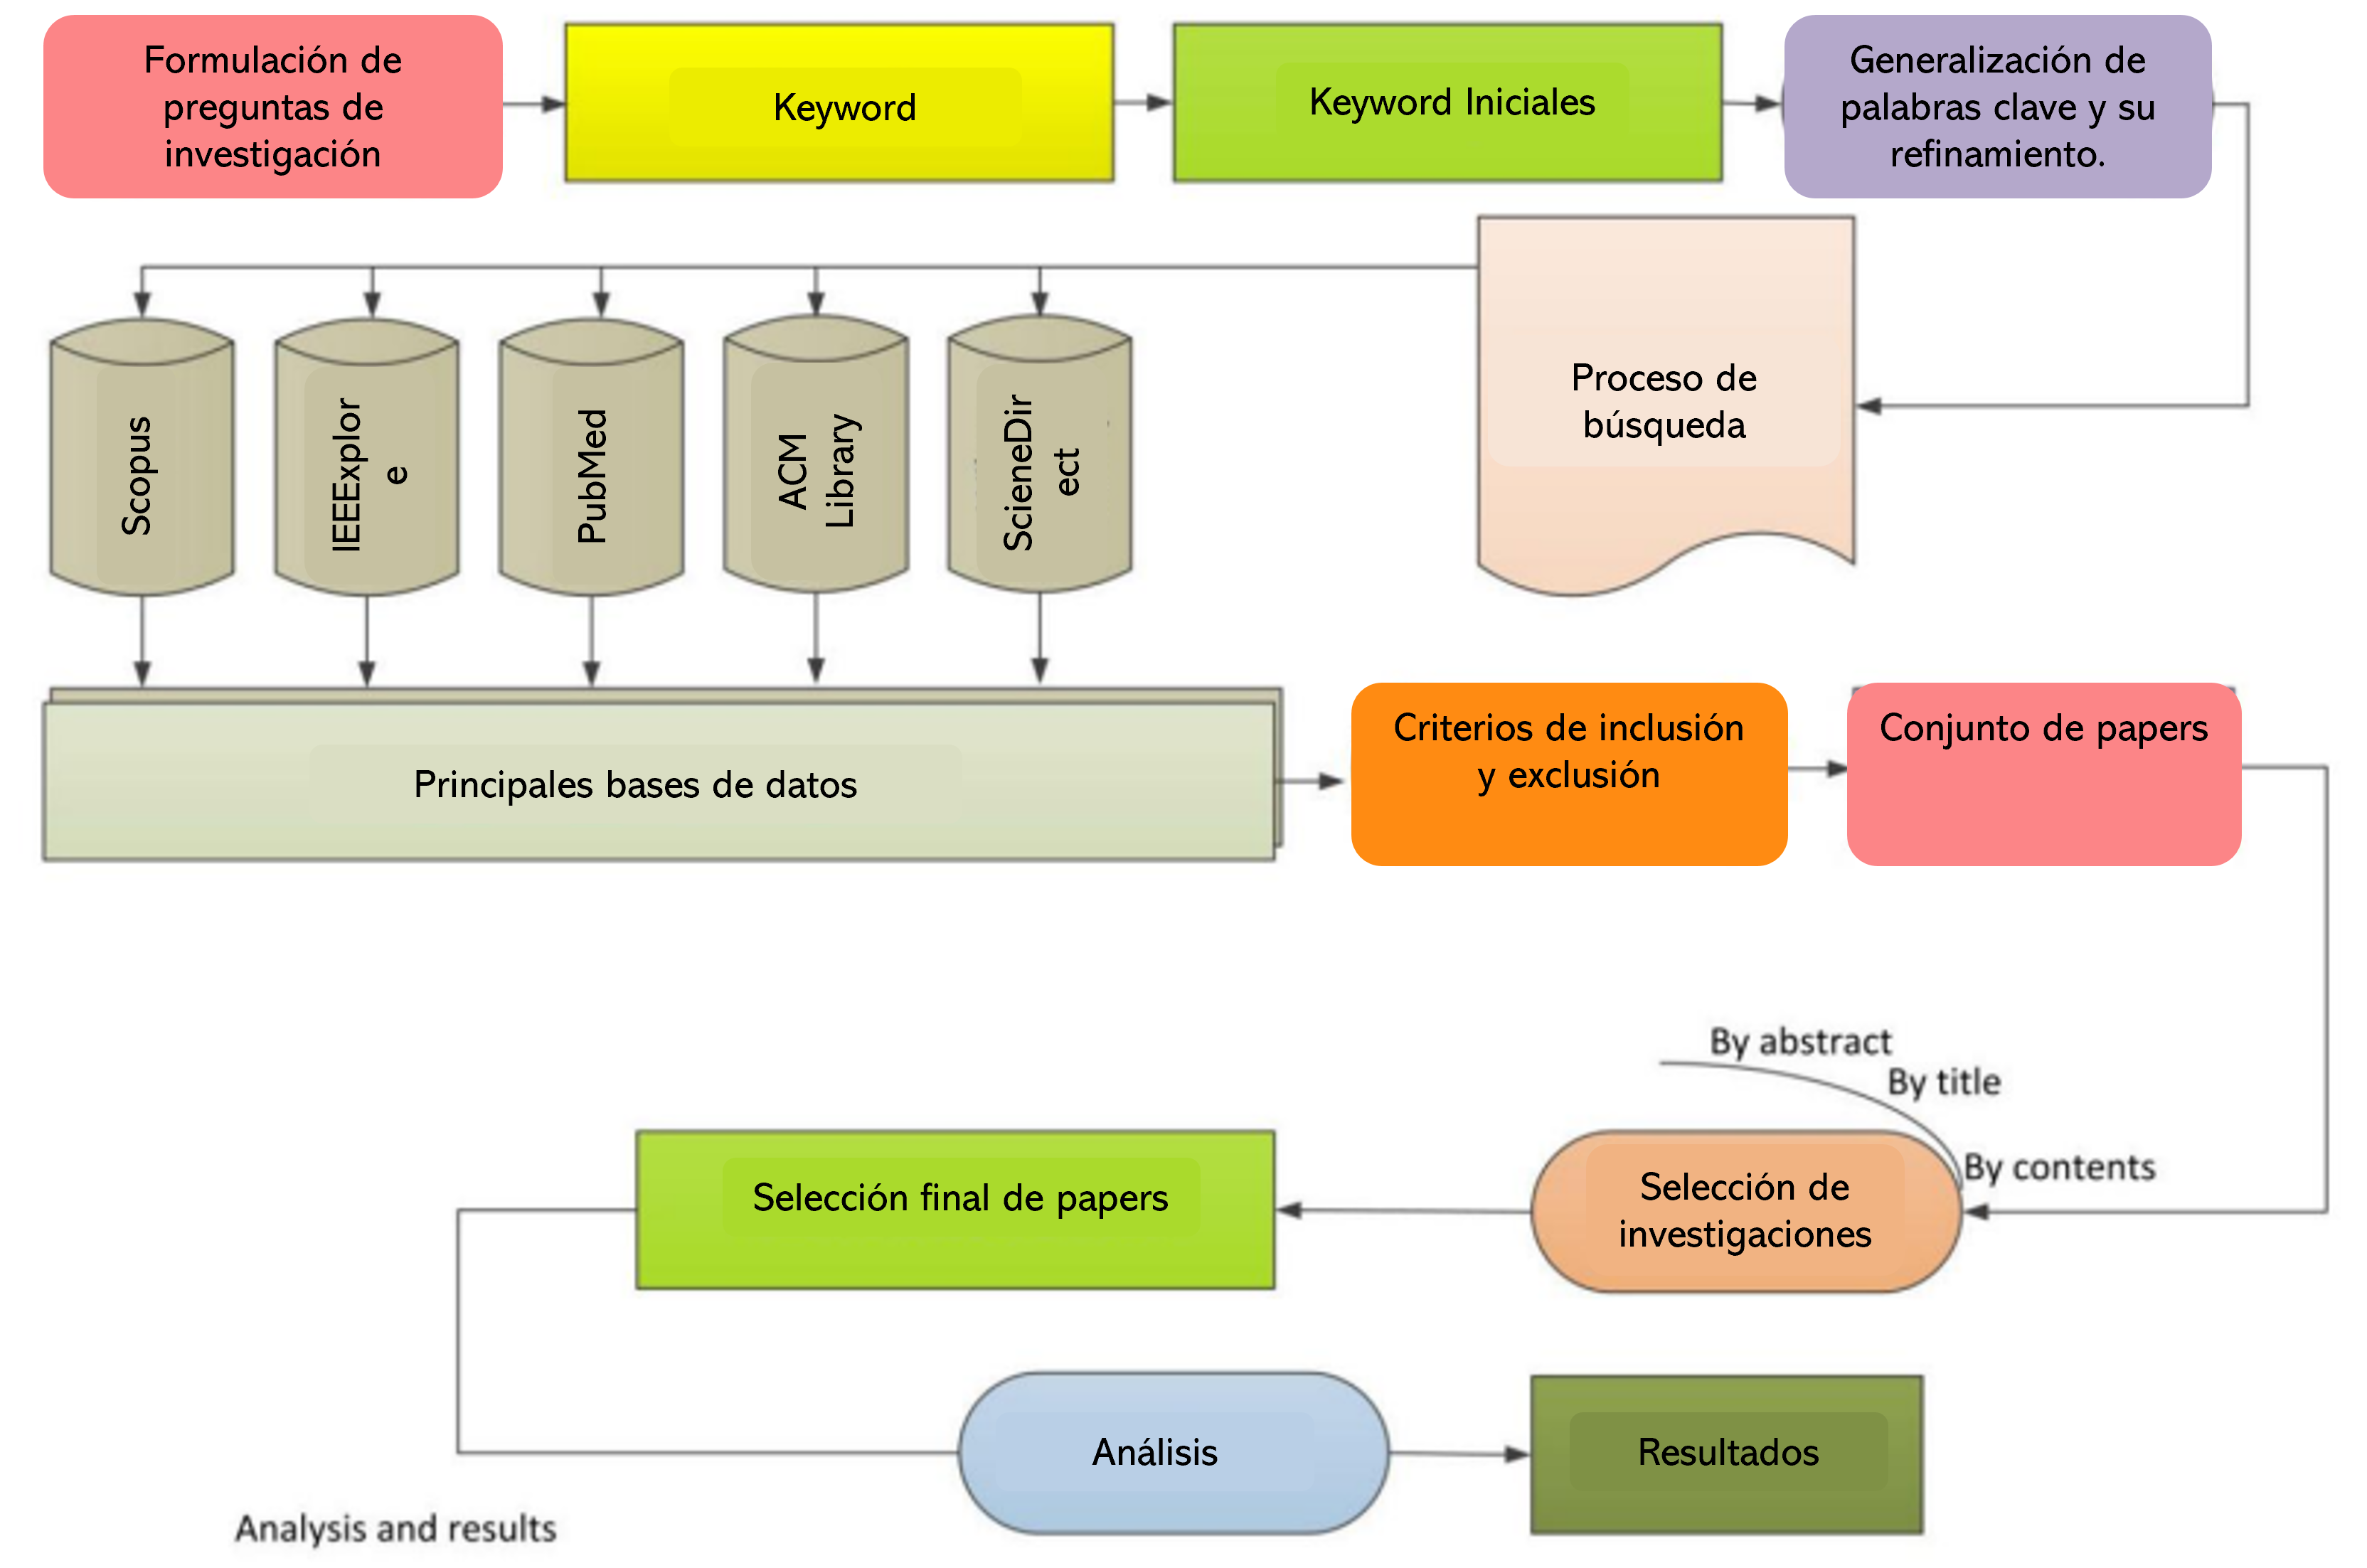
\includegraphics[width=1\columnwidth]{graficos/protocolo-seguido.png}
    		\caption{Protocolo de seleccion de estudios significativos.}
    		\label{operadores}
    	\end{figure}
 
	\subsection{Preguntas de investigación}
	Para abordar la complejidad de la aplicación de la visión computacional en la mejora de la movilidad de personas con discapacidad visual, es fundamental plantear preguntas de investigación que guíen este análisis. En este contexto, las siguientes preguntas clave se plantean para explorar en profundidad el estado actual de esta tecnología, sus aplicaciones, limitaciones y su impacto en la vida cotidiana de las personas con discapacidad visual:
    \begin{itemize}
        \item ¿Cuáles son las soluciones tecnológicas de visión computacional más relevantes para la identificación de objetos en la movilidad de personas con discapacidad visual?
        \item ¿Qué metodologías y técnicas se utilizan comúnmente en la aplicación de visión computacional para ayudar a las personas con discapacidad visual?
        \item ¿Qué tipos de interfaz de retroalimentación se han desarrollado para mejorar la experiencia del usuario con discapacidad visual?
        \item ¿Cuál es la eficacia de las soluciones de visión computacional en la mejora de la movilidad y la calidad de vida de las personas con discapacidad visual?
    \end{itemize}

	\subsection{Cadena de búsqueda}
	Para realizar una búsqueda efectiva de artículos relacionados con nuestro proyecto de revisión sistemática sobre la aplicación de visión computacional en la identificación de objetos para mejorar la movilidad de personas con discapacidad visual, es esencial identificar palabras clave pertinentes y construir una cadena de búsqueda estratégica. Las palabras clave se componen de términos representativos y relevantes que nos permitirán obtener respuestas de interés en motores de búsqueda de revistas científicas.
    Palabras clave identificadas:
    
    \begin{itemize}
        \item \textbf{\textit{En español: Visión Computacional, Identificación de Objetos, Movilidad, Discapacidad Visual, Dispositivos de Navegación, Tecnologías de Asistencia, Reconocimiento de Objetos, Navegacion personas.}}
        \item \textbf{\textit{En Ingles: Computer Vision, Object Identification, Mobility, Visual Disability, Navigation Devices, Assistive Technologies, Object Recognition, People Navigation.}}
    \end{itemize}
    
    El inglés es el idioma predominante en la comunidad científica, por lo que las palabras clave deben estar en inglés para garantizar la cobertura de la revisión sistemática.
    Utilizaremos estas palabras clave para construir una cadena de búsqueda efectiva. Para cada palabra clave individual, identificaremos sinónimos y los concatenaremos con el conector OR. Luego, combinaremos los grupos de palabras clave con el conector AND para crear una cadena de búsqueda completa, como se muestra en la Figura \ref{operadores}:
    
	\espkeywords 
    (''Visión por computadora'') AND (''Discapacidad visual'' OR ''Personas ciegas'') AND (''Detección de objetos'' OR ''Reconocimiento de objetos'' OR ''Sistema de navegación'')\\
	En ingles: \\
	\textbf{(''Computer Vision'') AND (''Visual Impairment'' OR ''Blind People'') AND (''Object Detection'' OR ''Object Recognition'' OR ''Navigation System'')}\\

    Esta cadena de búsqueda incluye las palabras clave relevantes y sus sinónimos. También utiliza operadores booleanos para combinar las palabras clave y restringir los resultados de la búsqueda a artículos que se relacionan con la visión computacional, la identificación de objetos, la movilidad de personas con discapacidad visual, la interacción y la retroalimentación, y el entorno.

    La tabla \ref{vision-computacional} representa la relación entre la ''Visión Computacional'' como variable independiente y la ''Movilidad de personas con Discapacidad Visual'' como variable dependiente. Proporciona términos de búsqueda relevantes que se utilizan para buscar investigaciones relacionadas con la aplicación de la visión computacional para mejorar la movilidad de personas con discapacidad visual a través de la detección de objetos. Los términos de búsqueda incluyen conceptos clave como ''Computer Vision'', ''Visual impairment'', ''Object Detection'', ''Visual Impaired'', ''Obstacle Detection'', ''Blind People'', ''Object recognition'', ''People navigate'', ''Obstacle detectors'' y ''Visual Assistance''.

    Estos términos de búsqueda se utilizan para identificar investigaciones y estudios que aborden la detección de objetos y la visión computacional en el contexto de la movilidad de personas con discapacidad visual, lo que es esencial para comprender y mejorar la vida de estas personas.

    \begin{table*}[hbtp]
    \centering
    \begin{tabular}{@{}cc@{}} \toprule
        \multicolumn{2}{c}{\textbf{Aplicación de la visión computacional para la mejora de la}} \\ 
        \multicolumn{2}{c}{\textbf{ movilidad de personas con discapacidad visual mediante la detección de objetos}} \\ \midrule
        \multicolumn{1}{c}{\textbf{Variable Independiente}} & \multicolumn{1}{c}{\textbf{Variable Dependiente}} \\ \midrule
        Vision Computacional & Movilidad de personas con Discapacidad Visual \\
        & \\
        \toprule
        \multicolumn{2}{c}{\textbf{Términos de Búsqueda}} \\ \midrule
        Computer Vision & Visual impairment  \\
        Object Detection & Visual Impaired  \\
        Obstacle Detection & Blind People  \\
        Object recognition & People navigate  \\
        Obstacle detectors & Visual Assistance  \\ \bottomrule
    \end{tabular}
    \caption{Variables y Términos de búsqueda.}
    \label{vision-computacional}
\end{table*}

    Esta cadena de búsqueda se utilizará en motores de búsqueda de bases de datos académicas relevantes para obtener artículos científicos relacionados con nuestra investigación. También se pueden agregar términos específicos o sinónimos según sea necesario para ajustar la búsqueda y obtener resultados más precisos.

    \begin{figure}[hbtp]
    		\centering
    		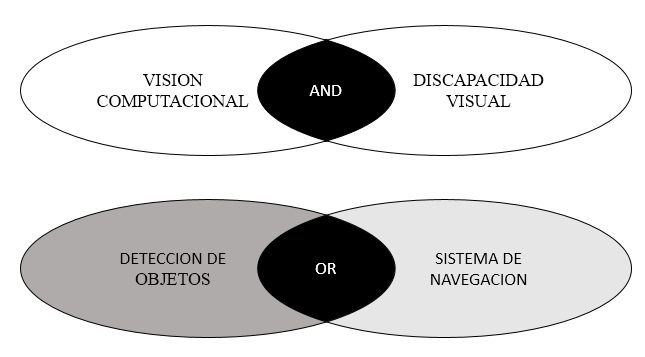
\includegraphics[width=1\columnwidth]{graficos/Operadores-booleanos.png}
    		\caption{Operadores Booleanos AND-OR.}
    		\label{operadores}
    	\end{figure}
	
	\subsection{Motores de búsqueda}
	La elección adecuada de motores de búsqueda y fuentes de artículos científicos es un paso crucial en el proceso de revisión sistemática. En particular, es importante considerar la calidad de la literatura recuperada, ya que esto puede afectar la validez de los resultados de la revisión. En el ámbito de la ciencia de la computación, existen dos enfoques principales para recuperar la literatura relevante:
    \begin{itemize}
        \item 1. Búsqueda en Google Academico: Este enfoque es rápido y fácil de usar, pero puede resultar en la inclusión de literatura no revisada por pares y metadatos de baja calidad.

        \item 2. Búsqueda en catálogos especializados: Este enfoque es más laborioso, pero ofrece una mayor garantía de calidad. Los catálogos especializados suelen incluir solo literatura revisada por pares y metadatos de alta calidad.
    \end{itemize}

En esta investigación, nos comprometemos con la calidad de la literatura recuperada. Por lo tanto, seleccionamos los siguientes motores de búsqueda y fuentes de artículos científicos:
	\begin{itemize}
	    \item ACM (\url{dl.acm.org})
        \item IEEE Xplore (\url{ieeexplore.ieee.org})
        \item Scopus (\url{scopus.com})
        \item PubMed (\url{pubmed.ncbi.nlm.nih.gov/})
        \item ScienceDirect (\url{www.sciencedirect.com})
    \end{itemize}
    
	\subsection{Refinamiento de cadena}
	En los motores de búsqueda definidos en la sección anterior, se ejecutó la cadena de palabras clave propuestas en la sección de cadena de búsqueda. Los resultados se presentan en la Tabla \ref{busqueda1}, donde el orden de la lista se basa en la relevancia de las revistas científicas y corresponde al período 2019 - 2023.
 
Sin perder de vista nuestro objetivo principal, que es la identificación de objetos en la movilidad de personas con discapacidad visual a través de la visión computacional, las palabras clave más relevantes para nuestro objetivo son ''Computer vision'' y ''visual disability''. Por lo tanto, estos términos no pueden ser excluidos al refinar nuestra cadena de búsqueda. Un segundo punto importante es tener en cuenta los idiomas en los que podemos realizar las busquedas en nuestra investigación, en este caso, ''ingles'', ''portugues'' y ''español''. 

Realizamos una búsqueda inicial y notamos que en el campo de investigación de la visión computacional para la identificación de objetos en la movilidad de personas con discapacidad visual, hay presencia de 2  revistas relacionadas a nuestro tema, por lo tanto, la palabra clave utilizada en las siguientes búsquedas será ''Visual impairment'' en lo que respecta a las personas con discapacidad visual, ya que fue una de las palabras observadas en el keyword de los unicos 2 articulos encontrados inicialmente.

Las cadenas de búsqueda final, que se basa en la Tabla \ref{busqueda1}, es la siguiente:

''Computer vision'' AND ''Visual impairment'' AND ''Object recognition''.

\begin{table*}[hbtp]
    \centering
    \resizebox{1\textwidth}{!}{%
        \begin{tabular}{@{}ccccccc@{}}
        \toprule
        Ingles & Scopus & PubMed & IEEExplore & ACM & ScienceDirect \\
        \midrule
        "Computer vision" AND "visual impairment" AND "object recognition" & 121 & 182 & 54 & 1947 & 1575 \\
        "Computer vision" AND "visual impaired" AND "object recognition" AND "People navigate" & 14 & 15 & 10 & 247 & 344 \\
        "Obstacle detection" AND "blind people" AND "People navigate" & 65 & 51 & 52 & 1145 & 261 \\
        "Computer vision" AND "Object detection" AND "people navigate" & 30 & 23 & 53 & 1026 & 1116 \\
        "Computer vision" AND "Blind people" AND "People navigate" & 67 & 52 & 71 & 629 & 710 \\
        \textbf{SUBTOTAL} & \textbf{297} & \textbf{323} & \textbf{240} & \textbf{4994} & \textbf{4006} \\
        \textbf{TOTAL} & \multicolumn{5}{c}{\textbf{9860}} \\
        \bottomrule
        \end{tabular}%
    }
    \caption{Resultados de búsquedas en diferentes bases de datos utilizando términos clave.}
    \label{busqueda1}
\end{table*}



Con una cadena de busqueda mas especializada tambien se obtienen los siguientes resultados como se muestra en la Tabla \ref{busqueda2}

\begin{table*}[hbtp]
    \centering
    \resizebox{1\textwidth}{!}{%
        \begin{tabular}{@{}ccccccc@{}}
        \toprule
        Ingles & Scopus & PubMed & IEEExplore & ACM & ScienceDirect \\
        \midrule
        ("Computer Vision") AND ("Visual Impairment" OR "Blind People") AND ("Object Detection" OR "Object Recognition" OR "Navigation System") & 47 & 252 & 178 & 337 & 159 \\
        \textbf{TOTAL} & \multicolumn{5}{c}{\textbf{973}} \\
        \bottomrule
        \end{tabular}%
    }
    \caption{Resultados de búsquedas en diferentes bases de datos utilizando términos clave.}
    \label{busqueda2}
\end{table*}


Realizando una búsqueda en bases de datos académicas, esperamos encontrar estudios relacionados con la aplicación de la visión computacional para la identificación de objetos en la movilidad de personas con discapacidad visual. Esta cadena de búsqueda se ajusta a nuestro objetivo de investigación y busca resultados específicos y relevantes.

    
    
	\subsection{Ejecución de búsqueda}
	En esta sección, documentaremos los resultados obtenidos con la cadena de búsqueda redefinida para nuestro tema de "Visión computacional para la identificación de objetos en la movilidad de personas con discapacidad visual", los cuales se presentarán en la Tabla \ref{busqueda3}. Las siguientes búsquedas tienen un filtro de artículos desde el año 2019 a 2023, ya que notamos que en los trabajos científicos relacionados con nuestra área de investigación, la relevancia se ha incrementado durante ese período, como se muestra en la Figura \ref{años}. También es importante aclarar que en el presente análisis se tomaron en cuenta los 100 primeros resultados según el orden de relevancia creado por los mismos motores de búsqueda.

A continuación, analizaremos los resultados de cada motor de búsqueda:
	\begin{figure}[hbtp]
    		\centering
    		\includegraphics[width=1\columnwidth]{graficos/Años.jpg}
    		\caption{Rango de año de publicación de artículos relacionados a las palabras clave}
    		\label{años}
    \end{figure}
	\subsubsection{Scopus}
    Con respecto a a la ejecución de la cadena de búsqueda en el motor de busqueda de Scopus, se encontró un total de 21 periódicos y 126 conferencias.
En la Figura \ref{cloud_w1} se aprecia la nube de palabras mas frecuentes en los textos de abstact, keywords y titulo, en donde: se evidencia la presencia de los términos referentes a nuestro objetivo, por ejemplo: object, visually impaired, object detection, computer vision, recognition, blind people,etc. 
Esto indica que los documentos recuperados están vinculados directamente con la temática de la visión computacional para la identificación de objetos en el contexto de la movilidad de personas con discapacidad visual.

    	\begin{figure}[H]
    		\centering
    		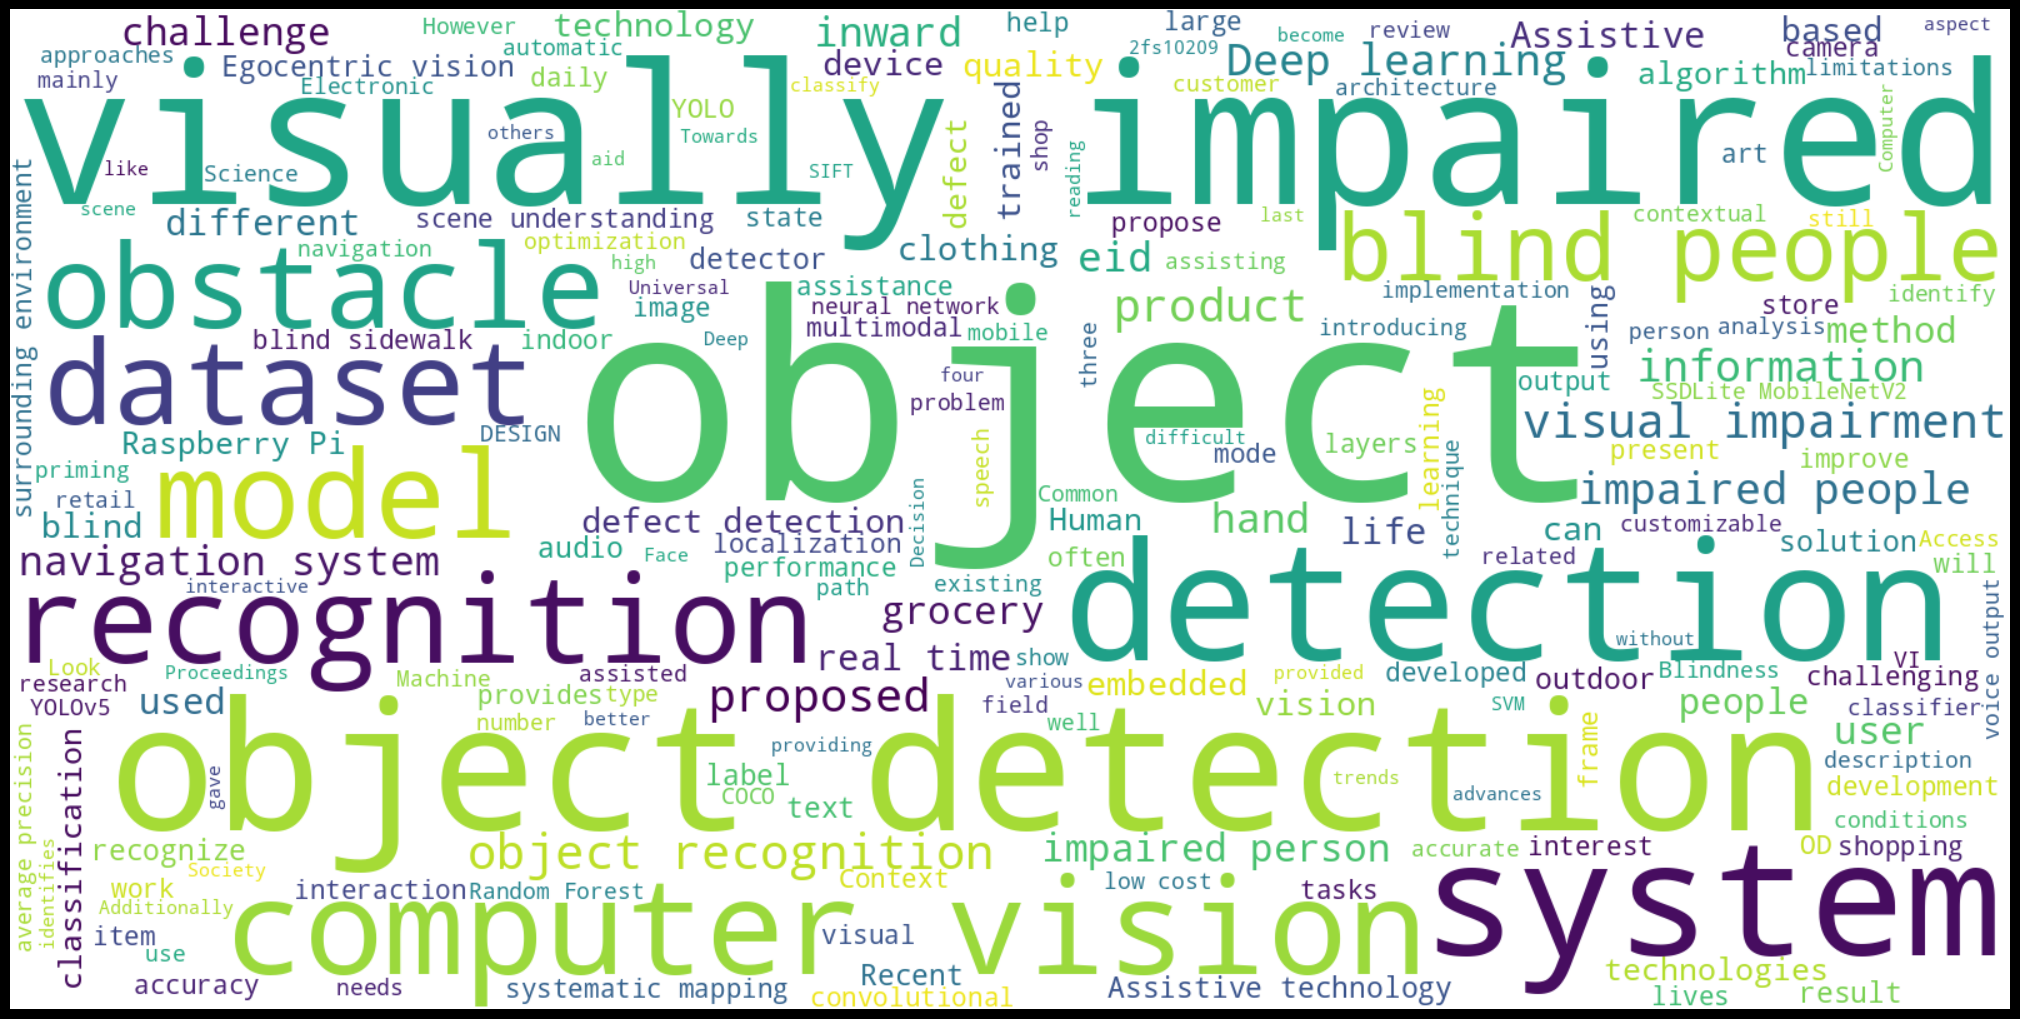
\includegraphics[width=1\columnwidth]{graficos/Scopus-nube.png}
    		\caption{Nube de palabras de textos de campo titulo, abstract y keywords de revistas encontrados en Scopus.}
    		\label{cloud_w1}
    	\end{figure}

Este análisis de la nube de palabras ayuda a confirmar que los documentos seleccionados están alineados con el enfoque de investigación y proporcionan una visión inicial de los conceptos y temas clave presentes en la literatura científica relevante.

	    \subsubsection{PubMed}
    Con respecto a a la ejecución de la cadena de búsqueda en el motor de busqueda de PubMed, se encontró un total de 6 periódicos y 87 conferencias.
En la Figura \ref{cloud_w2} se aprecia la nube de palabras mas frecuentes en los textos de abstact, keywords y titulo, en donde: se evidencia la presencia de los términos referentes a nuestro objetivo, por ejemplo: object, visual, people, vision, visually impaired, blind, recognition,etc. 

Esto indica que los documentos recuperados están vinculados directamente con la temática de la visión computacional para la identificación de objetos en el contexto de la movilidad de personas con discapacidad visual.

    	\begin{figure}[H]
    		\centering
    		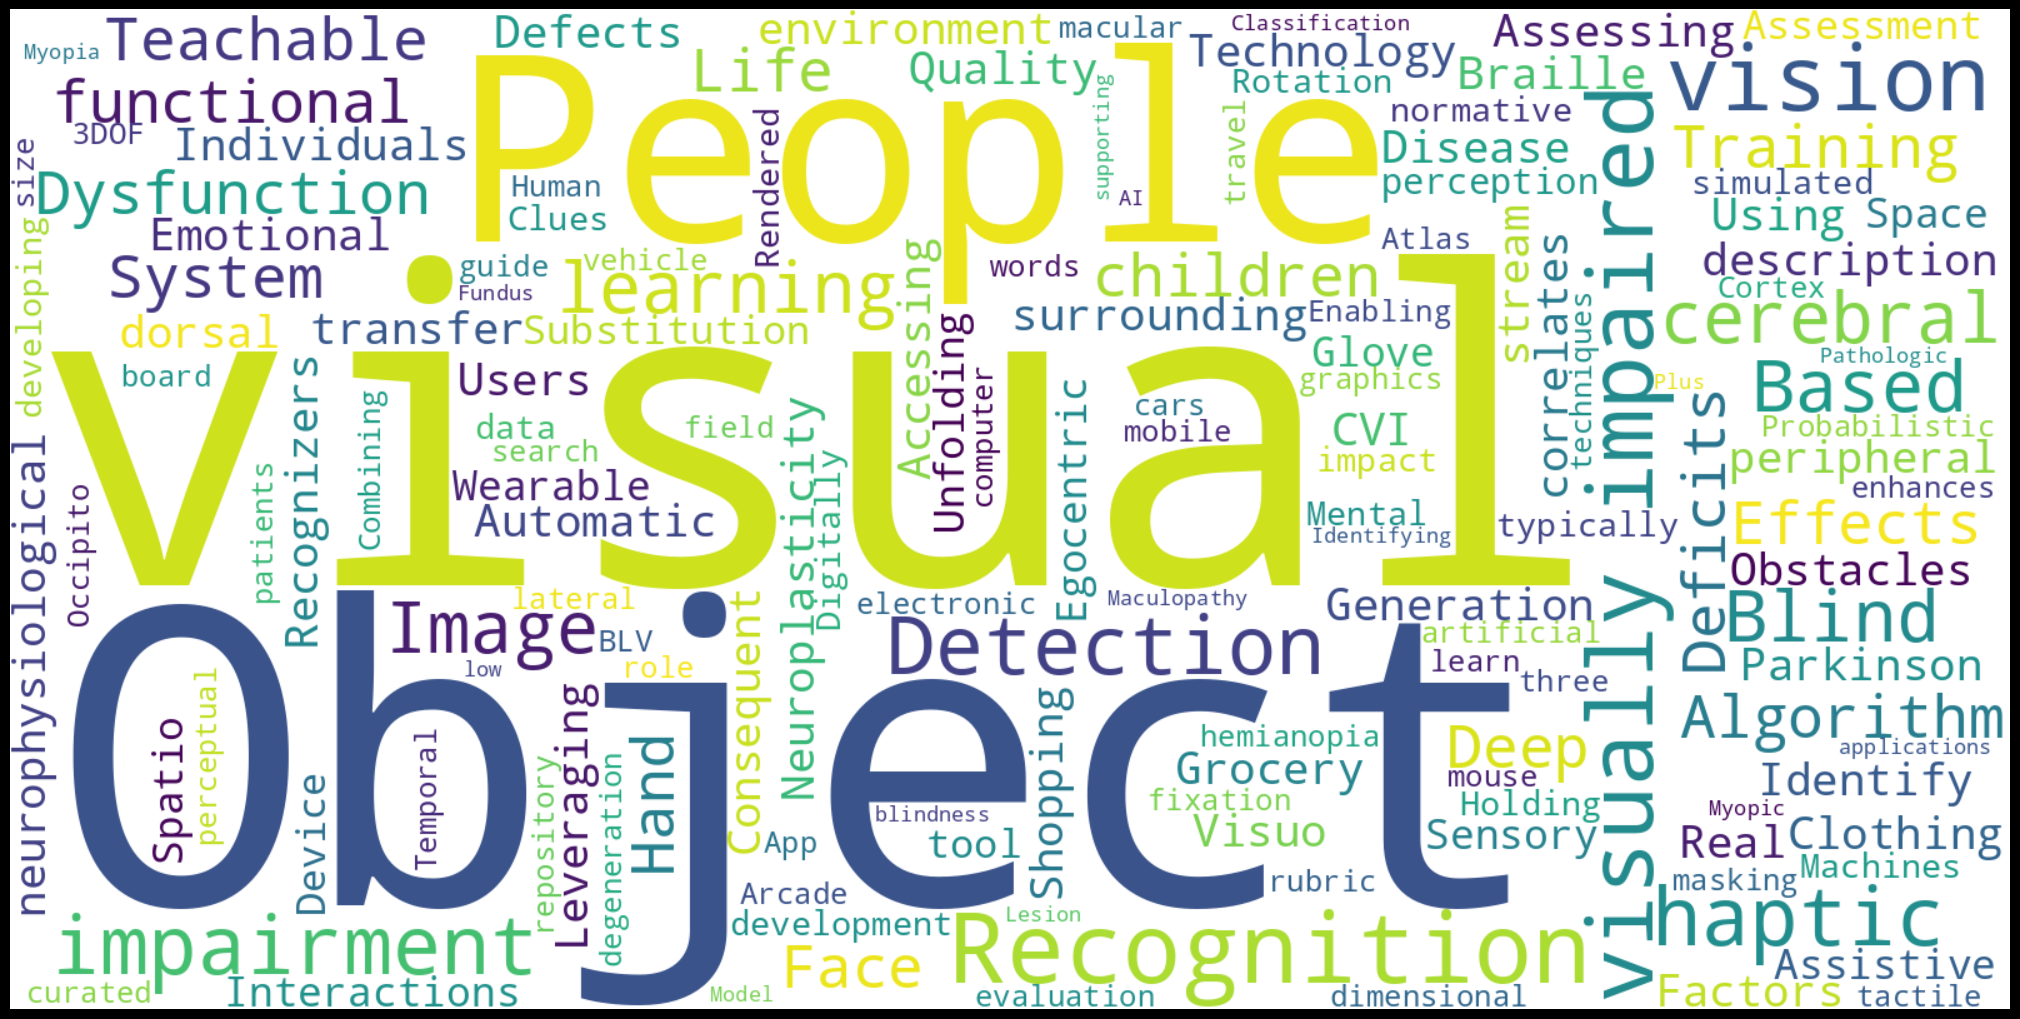
\includegraphics[width=1\columnwidth]{graficos/PubMed-nube.png}
    		\caption{Nube de palabras de textos de campo titulo, abstract y keywords de revistas encontrados en PubMed.}
    		\label{cloud_w2}
    	\end{figure}

Este análisis de la nube de palabras ayuda a confirmar que los documentos seleccionados están alineados con el enfoque de investigación.

\subsubsection{IEEExplore}
    Con respecto a a la ejecución de la cadena de búsqueda en el motor de busqueda de IEEExplore, se encontró un total de 64 periódicos y 70 conferencias.
En la Figura \ref{cloud_w3} se aprecia la nube de palabras mas frecuentes en los textos de abstact, keywords y titulo, en donde: se evidencia la presencia de los términos referentes a nuestro objetivo, por ejemplo: object detection, visually impaired, computer vision, system, blind people,visually impairment, etc. 
Esto indica que los documentos recuperados están vinculados directamente con la temática de la visión computacional para la identificación de objetos en el contexto de la movilidad de personas con discapacidad visual.

    	\begin{figure}[H]
    		\centering
    		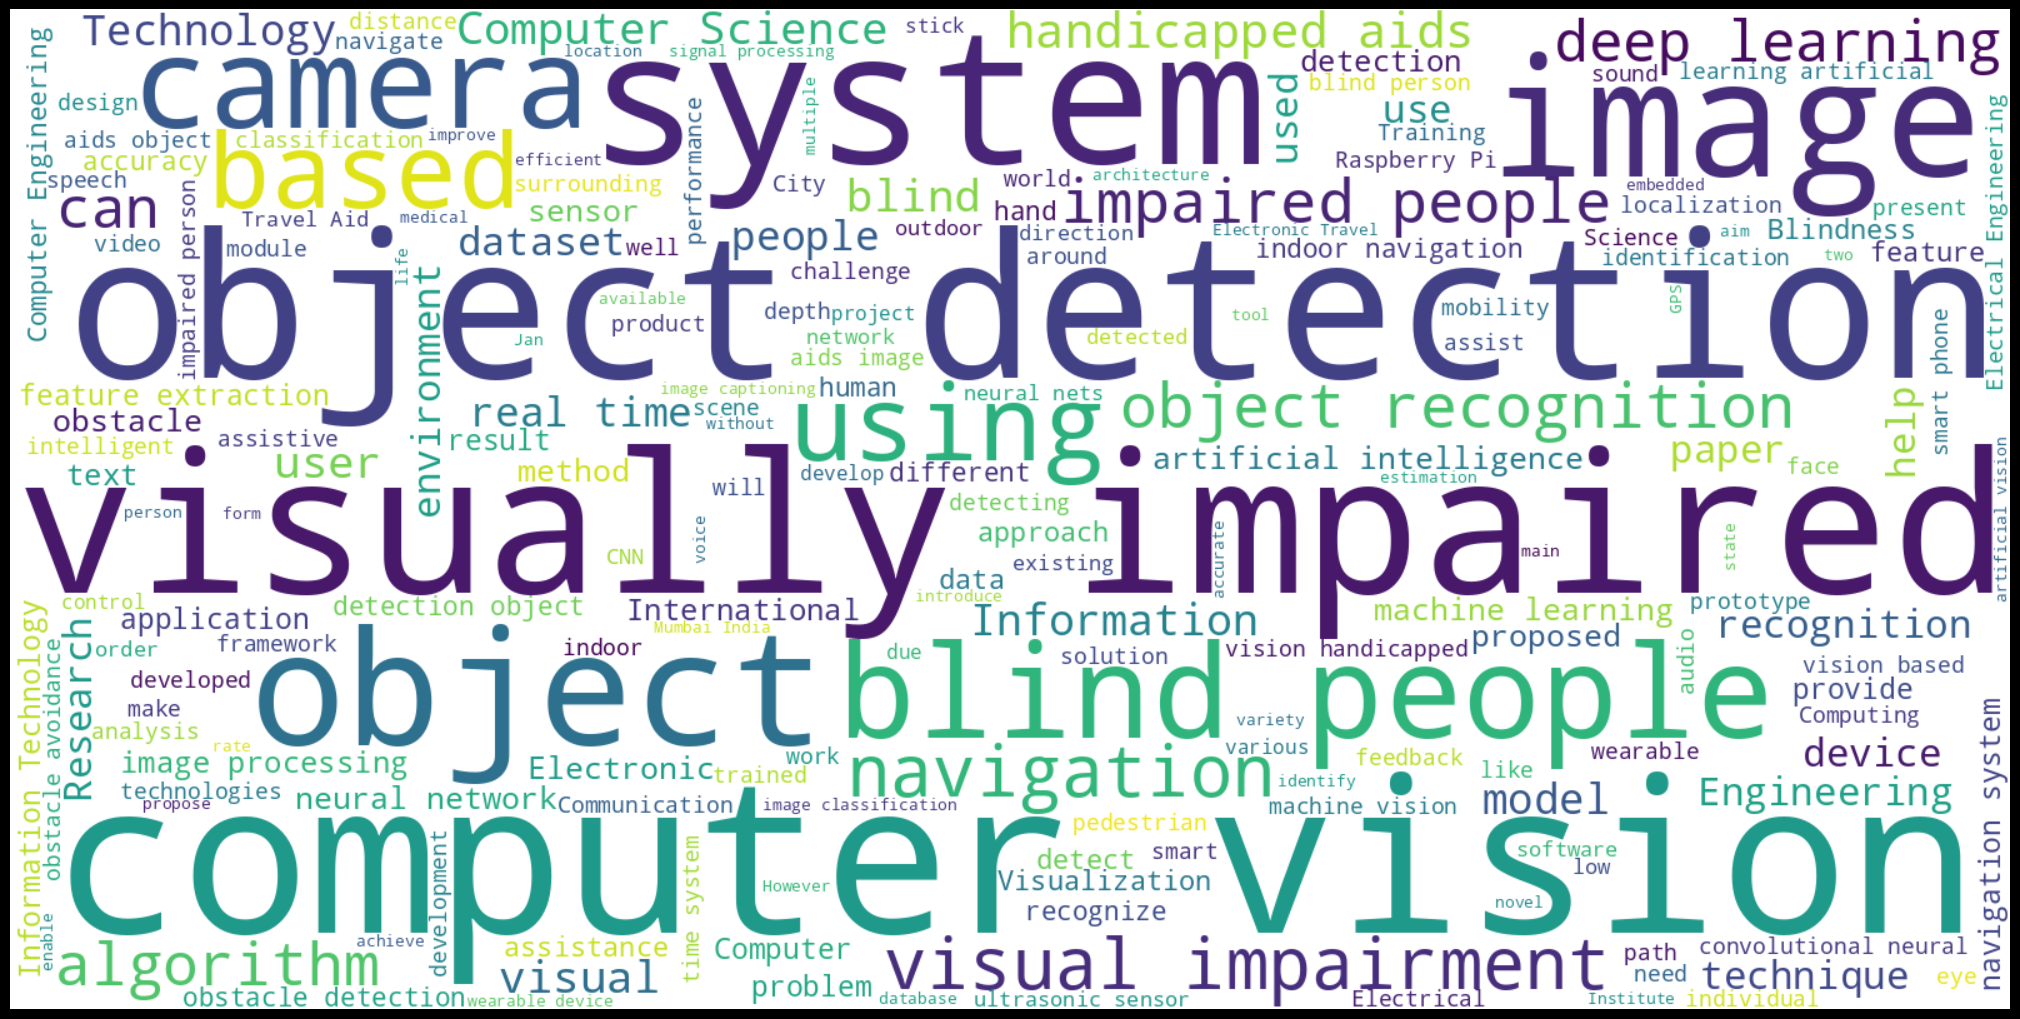
\includegraphics[width=1\columnwidth]{graficos/IEEE-nube.png}
    		\caption{Nube de palabras de textos de campo titulo, abstract y keywords de revistas encontrados en IEEExplore.}
    		\label{cloud_w3}
    	\end{figure}

Este análisis de la nube de palabras ayuda a confirmar que los documentos seleccionados están alineados con el enfoque de investigación y proporcionan una visión inicial de los conceptos y temas clave presentes en la literatura científica relevante.

\subsubsection{ACM Library}
    Con respecto a a la ejecución de la cadena de búsqueda en el motor de busqueda de ACM Library, se encontró un total de 211 periódicos y 198 conferencias.
En la Figura \ref{cloud_w4} se aprecia la nube de palabras mas frecuentes en los textos de abstact, keywords y titulo, en donde: se evidencia la presencia de los términos referentes a nuestro objetivo, por ejemplo: system, based, blind, people, visually impaired, blind people,etc. 
Esto indica que los documentos recuperados están vinculados directamente con la temática de la visión computacional para la identificación de objetos en el contexto de la movilidad de personas con discapacidad visual.

    	\begin{figure}[H]
    		\centering
    		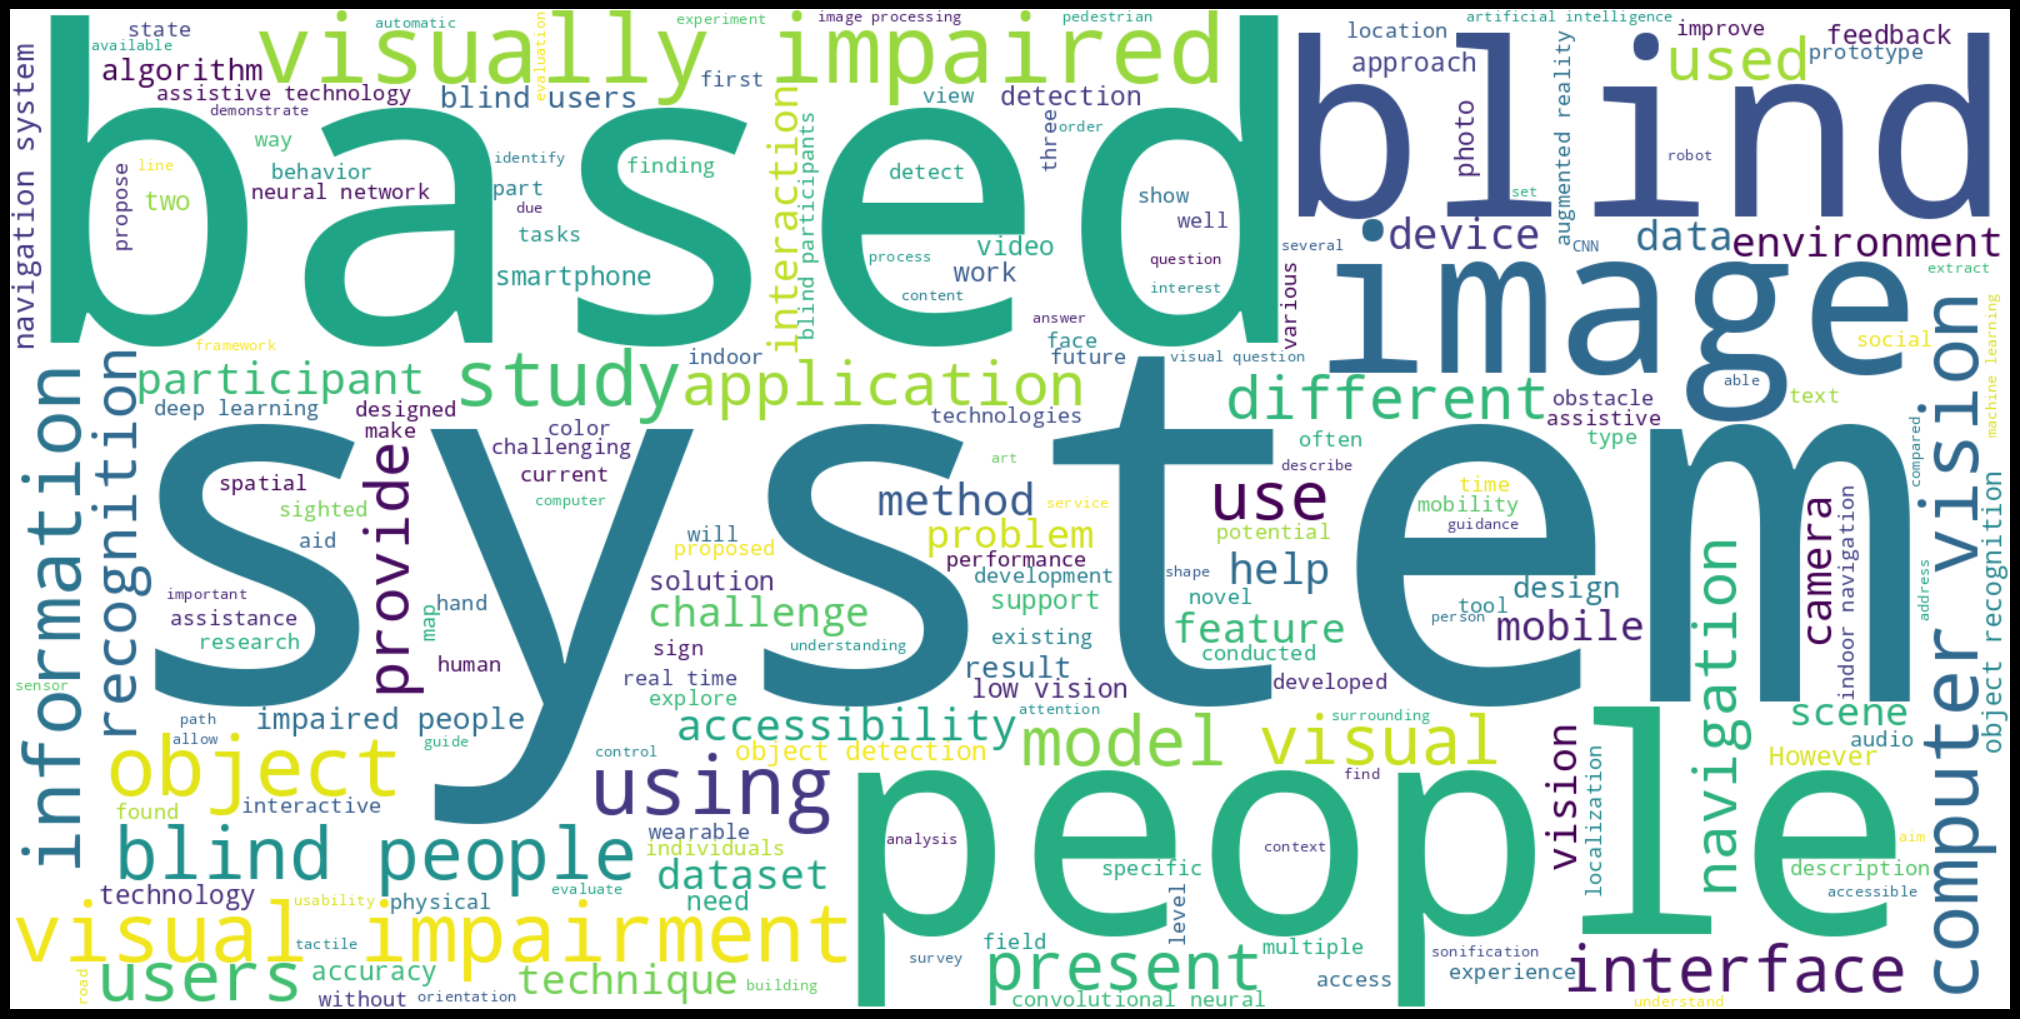
\includegraphics[width=1\columnwidth]{graficos/ACM-nube.png}
    		\caption{Nube de palabras de textos de campo titulo, abstract y keywords de revistas encontrados en ACM Library.}
    		\label{cloud_w4}
    	\end{figure}

Este análisis de la nube de palabras ayuda a confirmar que los documentos seleccionados están alineados con el enfoque de investigación y proporcionan una visión inicial de los conceptos y temas clave presentes en la literatura científica relevante.

 \subsubsection{ScienceDirect}
    Con respecto a a la ejecución de la cadena de búsqueda en el motor de busqueda de ScienceDirect, se encontró un total de 21 periódicos y 126 conferencias.
En la Figura \ref{cloud_w5} se aprecia la nube de palabras mas frecuentes en los textos de abstact, keywords y titulo, en donde: se evidencia la presencia de los términos referentes a nuestro objetivo, por ejemplo: visually impaired, navigation, model, system, object, vision, image,etc. 
Esto indica que los documentos recuperados están vinculados directamente con la temática de la visión computacional para la identificación de objetos en el contexto de la movilidad de personas con discapacidad visual.

    	\begin{figure}[H]
    		\centering
    		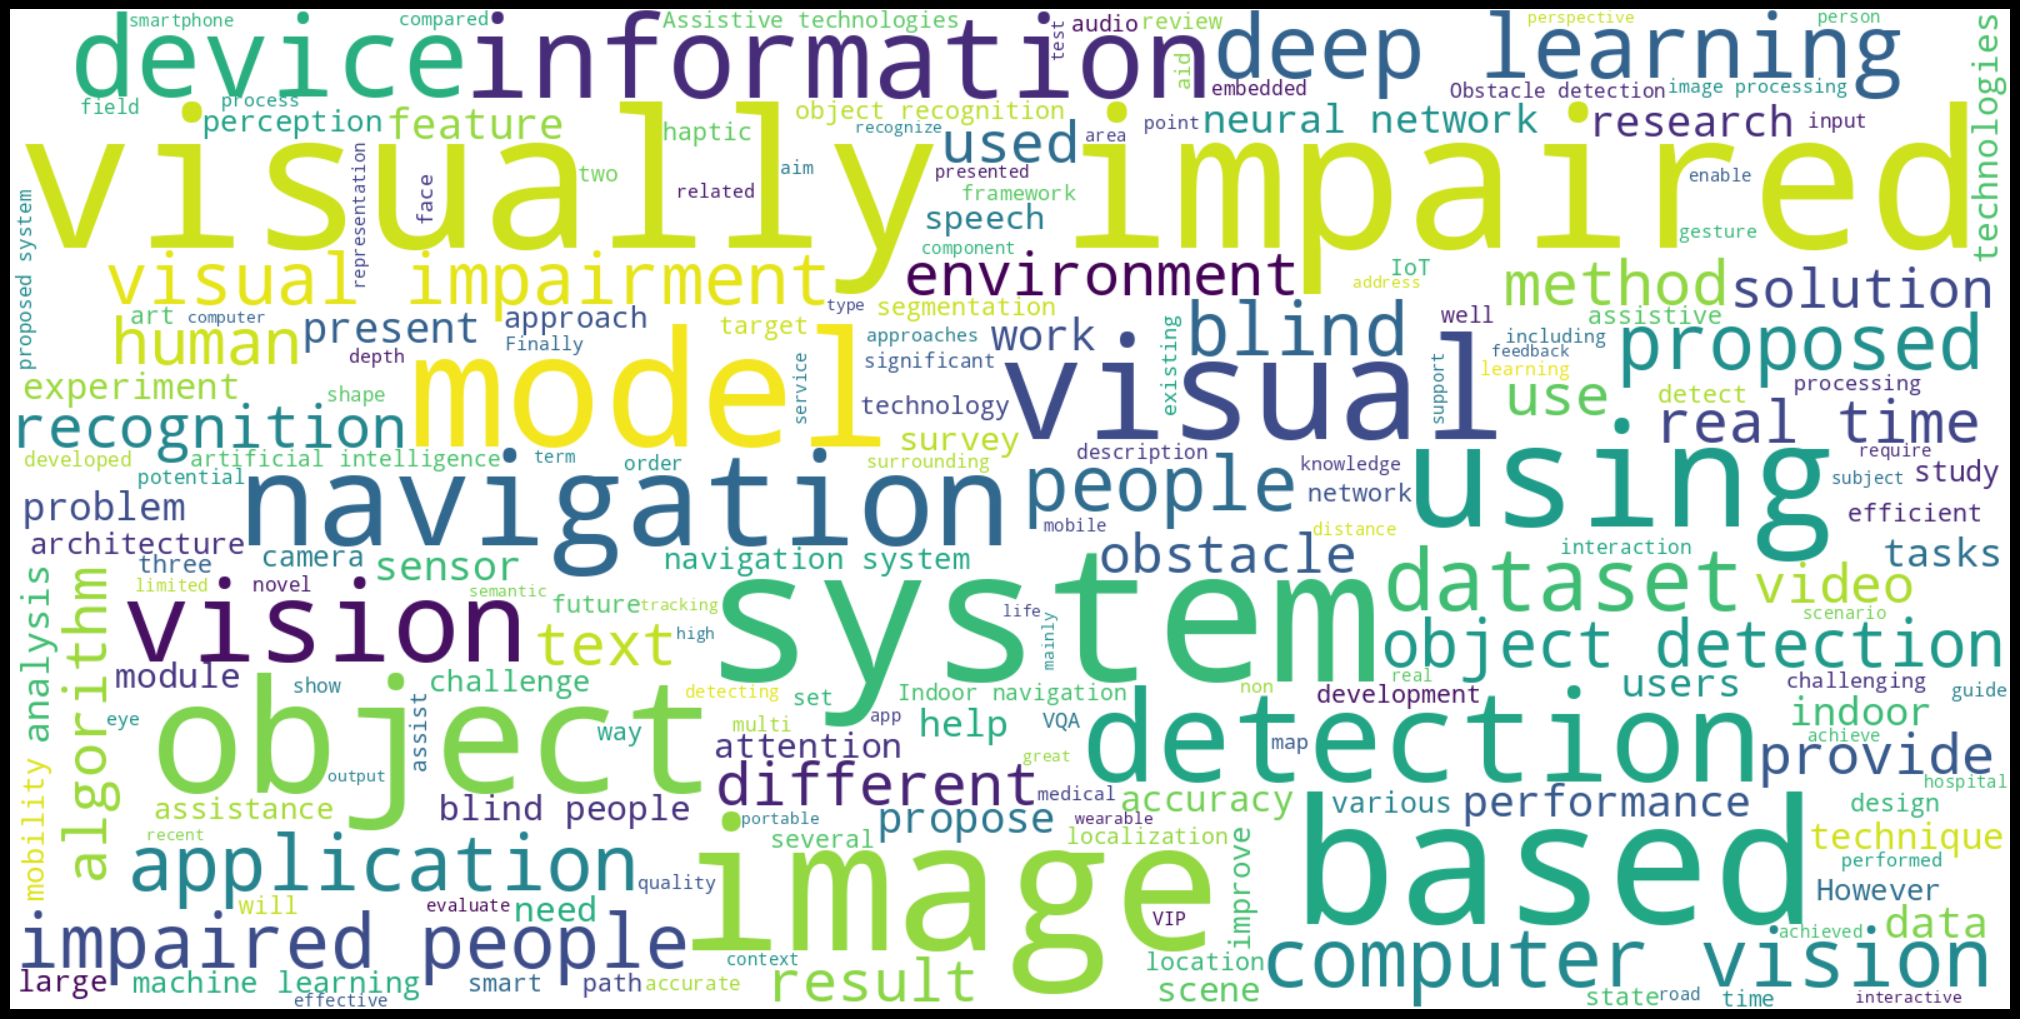
\includegraphics[width=1\columnwidth]{graficos/ScienceDirect-nube.png}
    		\caption{Nube de palabras de textos de campo titulo, abstract y keywords de revistas encontrados en ScienceDirect.}
    		\label{cloud_w5}
    	\end{figure}

Este análisis de la nube de palabras ayuda a confirmar que los documentos seleccionados están alineados con el enfoque de investigación y proporcionan una visión inicial de los conceptos y temas clave presentes en la literatura científica relevante.
En la tabla \ref{busqueda4} podemos ver el resumen en función de los motores de búsqueda y el tipo de revista encontrada.

\begin{table*}[hbtp]
    \centering
    \resizebox{1\textwidth}{!}{%
        \begin{tabular}{@{}ccccccc@{}}
        \toprule
        Ingles & Scopus & PubMed & IEEExplore & ACM & ScienceDirect \\
        \midrule
        "Computer vision" AND "visual impairment" AND "object recognition" & 59 & 24 & 39 & 98 & 255 \\
        "Computer vision" AND "visual impaired" AND "object recognition" AND "People navigate" & 8 & 8 & 7 & 18 & 43 \\
        "Obstacle detection" AND "blind people" AND "People navigate" & 35 & 24 & 26 & 129 & 30 \\
        "Computer vision" AND "Object detection" AND "people navigate" & 16 & 10 & 33 & 56 & 159 \\
        "Computer vision" AND "Blind people" AND "People navigate" & 29 & 27 & 29 & 108 & 60 \\
        \textbf{SUBTOTAL} & \textbf{147} & \textbf{93} & \textbf{134} & \textbf{409} & \textbf{547} \\
        \textbf{TOTAL} & \multicolumn{5}{c}{\textbf{1330}} \\
        \bottomrule
        \end{tabular}%
    }
    \caption{Resultados de búsquedas en diferentes bases de datos utilizando términos clave.}
    \label{busqueda3}
\end{table*}

\begin{table*}[hbtp]
    		\centering
    		\begin{tabular}{@{}cll@{}} \toprule
    			\multicolumn{3}{c}{\textbf{Resumen de resultado}} \\ \midrule
    			Motor de búsqueda & Cantidad de revistas encontradas & periódico / conferencia \\ \midrule
                Scopus & 21 / 126 & Journals/Conferences \\
    			PubMed & 6 / 87 & Journals/Conferences \\
    			IEEE & 64 / 70 & Journals/Conferences \\
    			ACM & 211 / 198 & Journals/Conferences \\
    			ScienceDirect & 21 / 126 & Journals/Conferences \\ \bottomrule
    		\end{tabular}
    		\caption{Segundo resultado: Tabla de revistas científicas encontrados por motores de búsqueda.}
    		\label{busqueda4}
    	\end{table*}


 \subsection{Recopilación de la información}
 Durante la fase inicial de este proceso de revisión sistemática, se llevó a cabo una meticulosa recopilación de datos generales de los estudios identificados. Esta etapa fue esencial para establecer una base sólida de información basándonos en los criterios de la investigación.

 \subsubsection{Criterios de inclusión y exclusión}
 \subsubsection{Criterios de Inclusion}
Los criterios de inclusión se establecen para garantizar que la muestra sea representativa de la población general que se está estudiando. En el caso de nuestro proyecto, los criterios de inclusión son los siguientes:

\begin{itemize}
    \item \textbf{Relevancia Temática: }Las publicaciones deben abordar directamente la aplicación de la visión computacional para mejorar la movilidad de personas con discapacidad visual mediante la detección de objetos.
    \item \textbf{Tipo de publicación: }Solo se incluirán publicaciones científicas, como artículos de revistas y conferencias.
    \item \textbf{Idioma: }Las publicaciones deben estar escritas en inglés, español o portugués.
    \item \textbf{Criterios de búsqueda: }El título, abstract o keywords del artículo debe incluir las palabras clave relacionadas con ''visión computacional'', ''discapacitad visual'' y ''detección de objetos''.
    \item \textbf{Repositorios y bases de datos confiables: }Las publicaciones deben estar disponibles en bases de datos académicas y repositorios relevantes, como ACM, IEEE Xplore, Scopus, PubMed y ScienceDirect.
    \item \textbf{Período de tiempo: }Limitaremos la búsqueda a un período de tiempo específico, desde 2019 hasta la fecha actual, para asegurar la relevancia y actualidad de las publicaciones.
    \item \textbf{Número Mínimo de Citaciones: }Las publicaciones deben haber sido citadas un número mínimo de veces, al menos 1 vez, para ser consideradas en el estudio. 
\end{itemize}

\subsubsection{Criterios de Exclusion}

Los criterios de exclusión se establecen para eliminar las publicaciones que no son relevantes para el estudio. En el caso de nuestro proyecto, los criterios de exclusión son los siguientes:

\begin{itemize}
    \item \textbf{Irrelevancia Temática: }Se excluyen las publicaciones que no estén directamente relacionadas con el tema de investigación.
    \item \textbf{Publicaciones no Científicas: }Se excluyen publicaciones que no sean de naturaleza académica, como libros de divulgación, noticias, blogs y contenido no revisado por pares.
    \item \textbf{Idioma no Inglés, Portugues o Español: }Se excluyen publicaciones en idiomas distintos al inglés, portugues y al español debido a limitaciones en la capacidad de análisis.
    \item \textbf{Ausencia de Palabras Clave Relevantes: }Se excluyen publicaciones que no incluyan palabras clave relacionadas con ''visión computacional'', ''discapacitad visual'' y ''detección de objetos'' en el título, resumen o palabras clave.
    \item \textbf{Fuentes No Confiables: }Se excluyen publicaciones que no estén disponibles en bases de datos académicas y repositorios confiables, como ACM, IEEE Xplore, Scopus, PubMed y ScienceDirect.
    \item \textbf{Fecha de Publicación Fuera del Rango: }Se excluyen publicaciones que estén fuera del período de tiempo establecido para el estudio, publicaciones anteriores a 2019.
    \item \textbf{Número Insuficiente de Citaciones: }Se excluyen publicaciones que no hayan sido citadas al menos 1 vez, lo que ayuda a priorizar investigaciones que han recibido cierto grado de reconocimiento en la comunidad académica.
\end{itemize}

Los criterios de investigación presentados en esta sección proporcionan una guía clara para la selección de las publicaciones que serán analizadas en nuestro estudio. Estos criterios se basan en los objetivos del estudio y garantizarán que los resultados sean válidos y confiables. 

  \subsection{Clasificación de la información}
  Los criterios de inclusión han permitido identificar estudios que se centran en temas relevantes, como la comparación de diferentes algoritmos de detección de objetos, la combinación de la detección de objetos con la salida de voz, y el desarrollo de nuevos algoritmos de detección de objetos. 

En esta etapa crucial de la revisión sistemática, se llevó a cabo la clasificación de los estudios identificados previamente en la fase de recopilación de información. El objetivo principal de esta fase es organizar de manera efectiva los estudios en categorías o temas que estén estrechamente relacionados con los objetivos de nuestra revisión.

En la tabla \ref{clasificacion} se puede observar la clasificación definida para la evaluación.

\begin{table*}[hbtp]
    \centering
    \resizebox{1\textwidth}{!}{%
        \begin{tabular}{@{}ccccccc@{}}
        \toprule
        Categoría & Scopus & PubMed & IEEExplore & ACM & ScienceDirect & Total \\
        \midrule
        Comparación Algoritmos de Detección Objetos & 2 & 1 & 4 & 1 & 1 & 9 \\
        Detección + Salida de Voz & 2 & 2 & 6 & 3 & 0 & 13 \\
        Algoritmo Detección de Objetos & 1 & 0 & 3 & 0 & 0 & 4 \\
        Detección + Distancia/Orientación + Voz & 1 & 0 & 2 & 0 & 1 & 4 \\
        \textbf{TOTAL} & \textbf{6} & \textbf{3} & \textbf{15} & \textbf{4} & \textbf{2} & \textbf{30} \\
        \bottomrule
        \end{tabular}%
    }
    \caption{Resultados por categoría en diferentes bases de datos.}
    \label{clasificacion}
\end{table*}

En la Figura \ref{preseleccion}, se puede observar el proceso de selección de cada motor de búsqueda.

        \begin{figure}[H]
    		\centering
    		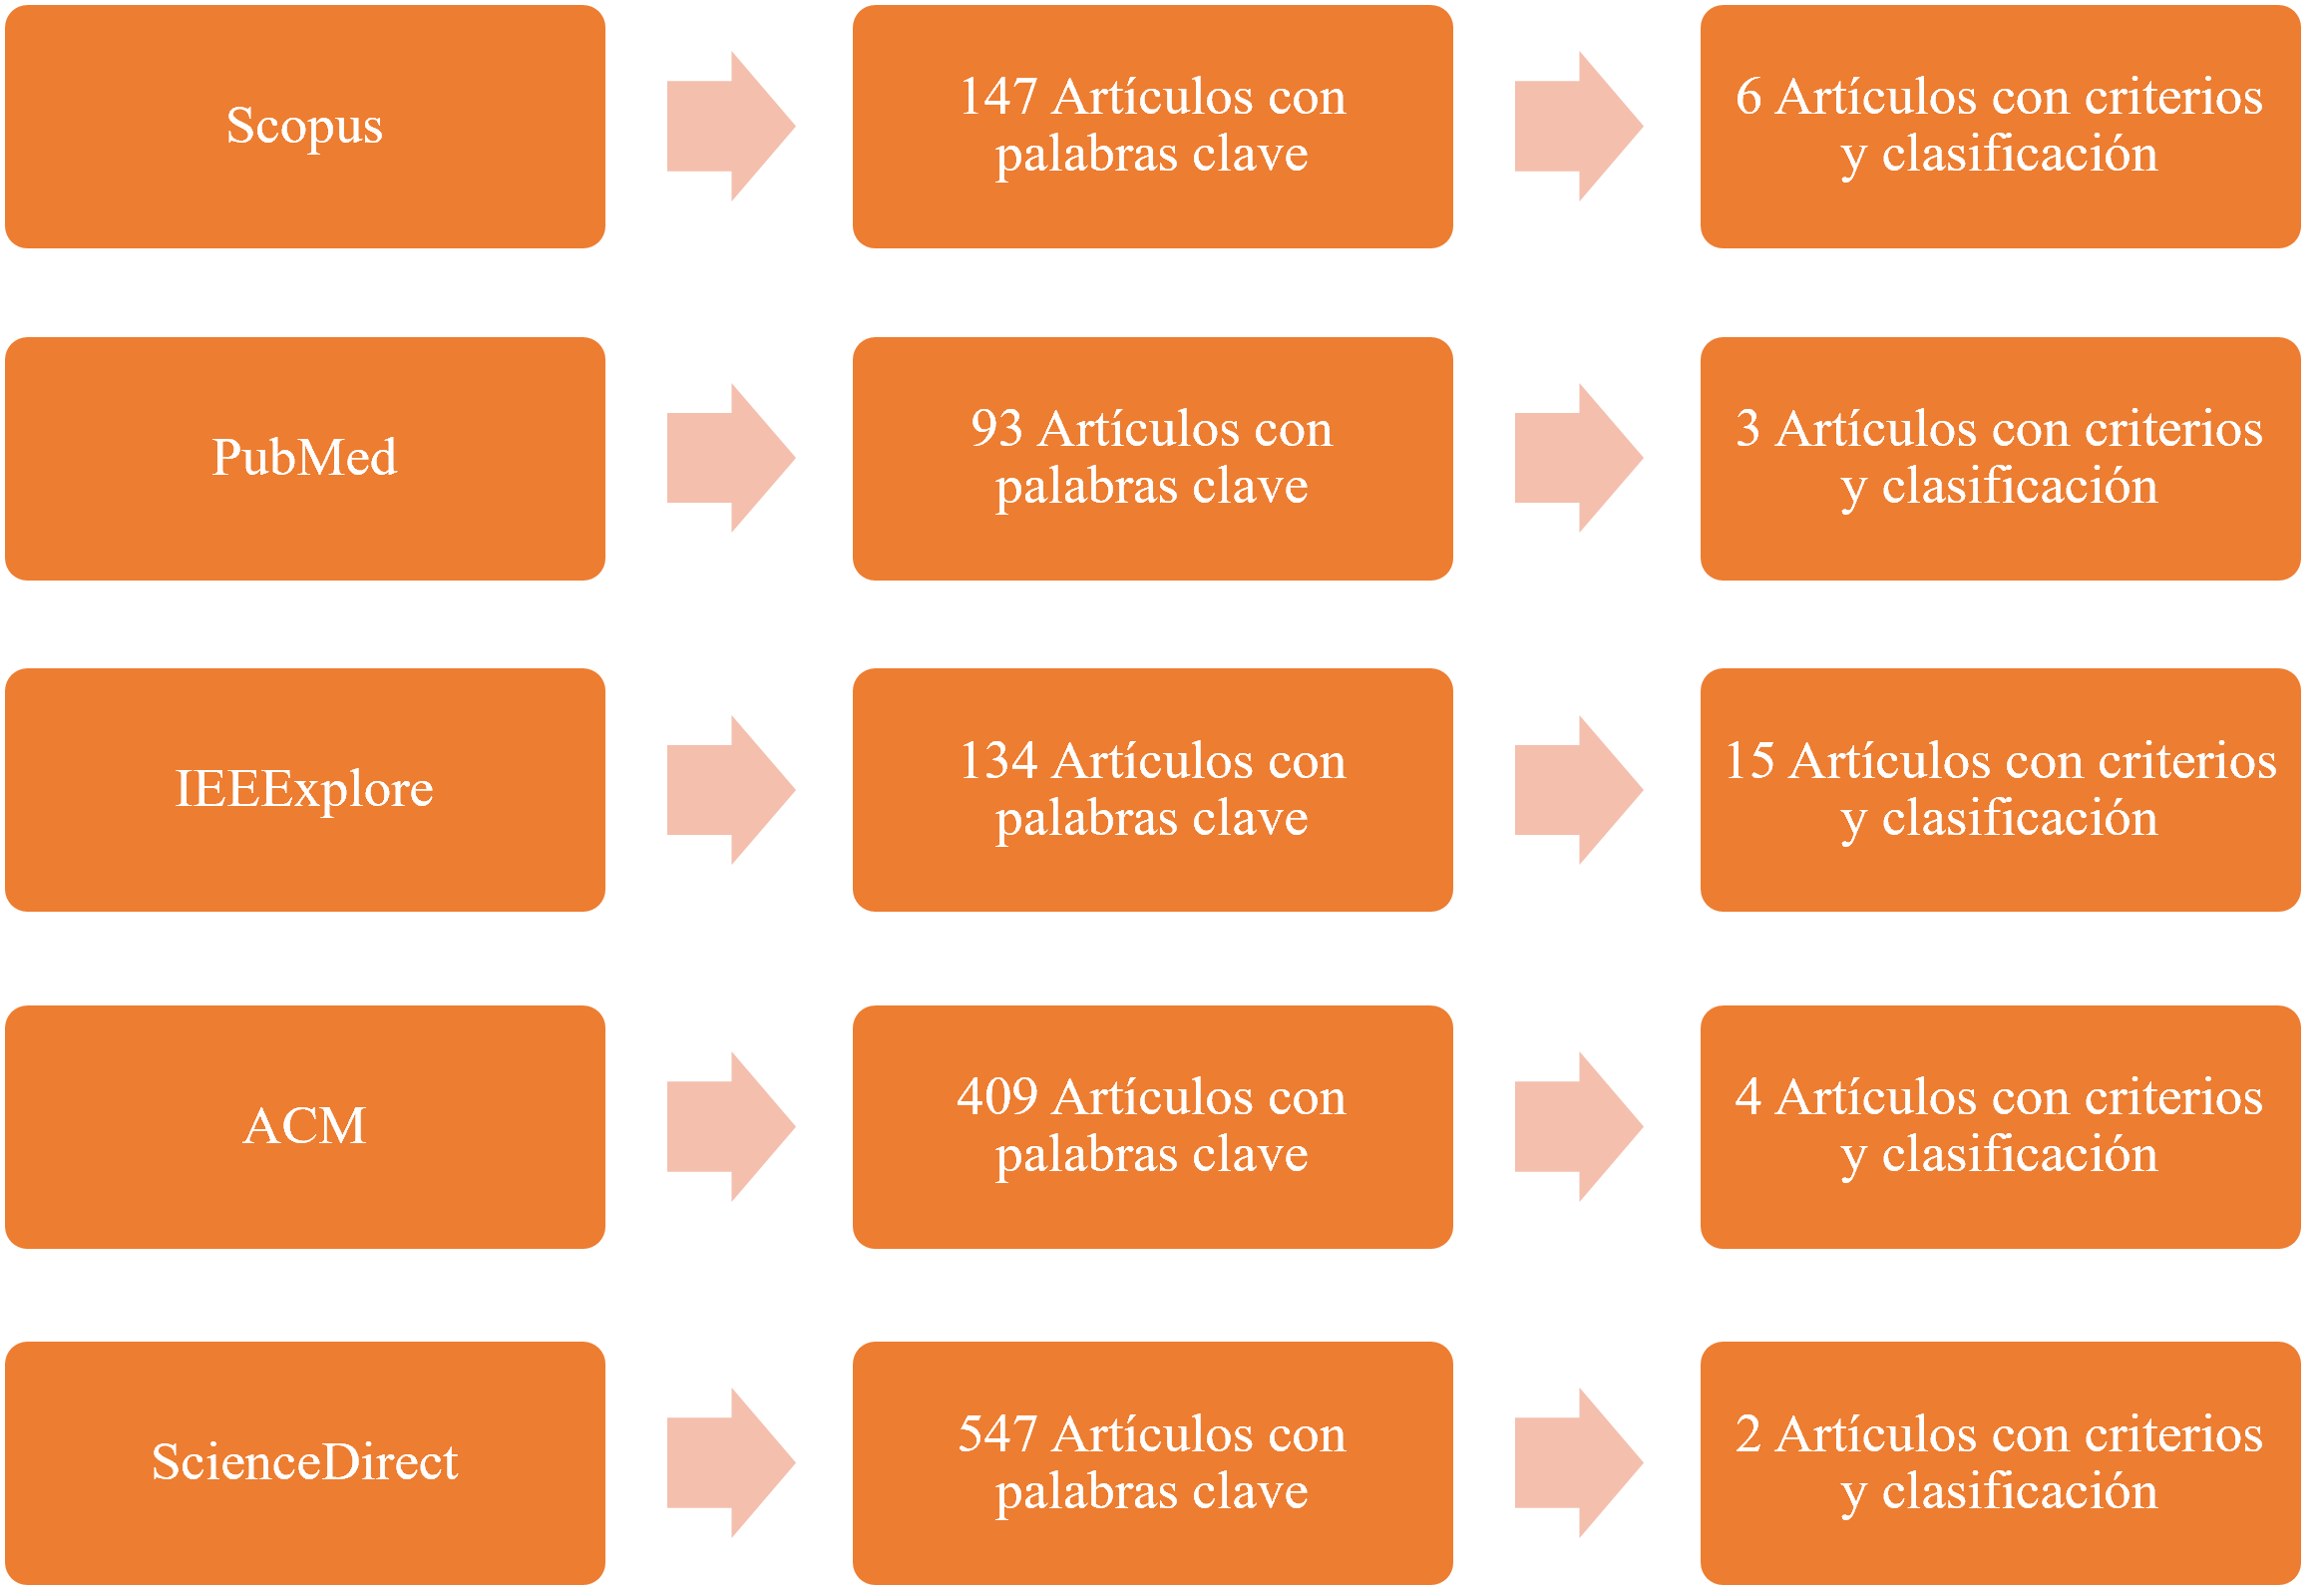
\includegraphics[width=1\columnwidth]{graficos/preseleccion.png}
    		\caption{Proceso Preliminar de Selección de Datos.}
    		\label{preseleccion}
    	\end{figure}

   \subsection{Discriminación por descarte}
   
La fase de discriminación por descarte, es fundamental para asegurar que solo los estudios más pertinentes y relevantes sean incluidos en nuestro análisis. Para llevar a cabo esta fase, aplicaremos la metodología PRISMA (Preferred Reporting Items for Systematic Reviews and Meta-Analyses), que proporciona una estructura sólida para realizar esta tarea de manera sistemática y transparente. En la siguiente tabla \ref{lista-verificacion}, se detallan los elementos que serán evaluados en cada estudio revisado, lo que incluye aspectos como el título, la justificación, el año de publicación, los objetivos, el diseño del estudio y otros factores críticos para garantizar la calidad y relevancia de los estudios seleccionados. Esta tabla se convertirá en una herramienta esencial para llevar a cabo una revisión sistemática exhaustiva y asegurar que los estudios incluidos contribuyan significativamente a la investigación en cuestión.
\begin{table*}[hbtp]
    \centering
    \resizebox{1\textwidth}{!}{%
        \begin{tabular}{@{}ccc@{}}
        \toprule
        SECCIÓN & ITEM & VERIFICACIÓN \\
        \midrule
        Título & 1 & Debe reflejar el contenido del estudio. \\
        Autor & 2 & Autores involucrados en el estudio. \\
        Año de Publicación & 3 & Año en que se publicó el estudio. \\
        Objetivo & 4 & Debe ser claro y específico, y debe indicar lo que se espera lograr con el estudio. \\
        Diseño del estudio & 5 & Debe describir el tipo de estudio que se realizó, incluidos los métodos y procedimientos utilizados. \\
        Componente o tecnología & 6 & Debe describir el componente o tecnología de visión computacional utilizado para la detección de objetos. \\
        Fuente de información & 7 & Debe indicar la base de datos, el número de imágenes y las clases utilizadas para entrenar el modelo. \\
        Interfaz de retroalimentación & 8 & Debe indicar qué tipo de retroalimentación se utilizó en el modelo o investigación. \\
        Área de Cobertura & 9 & Debe indicar el área de cobertura del modelo (interno o externo), es decir, área donde se aplicó la investigación. \\
        País & 10 & Debe indicar el país en el que se realizó el estudio. \\
        Resultados & 11 & Debe presentar los resultados del estudio, incluyendo la precisión, la sensibilidad y la especificidad del modelo. \\
        \bottomrule
        \end{tabular}%
    }
    \caption{Lista de verificación de elementos clave en el estudio de detección de objetos mediante visión computacional.}
    \label{lista-verificacion}
\end{table*}

    \subsection{Selección de estudios}
En esta sección llevamos a cabo un análisis detallado de los títulos y resúmenes de los estudios, aplicando los criterios previamente establecidos. Esta evaluación minuciosa fue esencial para determinar si cada estudio cumplía con los requisitos de relevancia y pertinencia exigidos por nuestra revisión sistemática, esta evaluacion la podemos observar en el Anexo \ref{anexo1}.

Se muestra en la Tabla \ref{analisis}, los estudios que cumplieron con la evaluación de los criterios de la Tabla \ref{lista-verificacion}.

\begin{table*}[hbtp]
    \centering
    \resizebox{1\textwidth}{!}{%
        \begin{tabular}{@{}cccccccccc@{}}
        \toprule
        Criterio y Evaluación & Artículo 1 & Artículo 2 & Artículo 3 & Artículo 4 & Artículo 5 \\
        \midrule
        ¿Tiene título acorde a la Investigación? & Sí & Sí & Sí & Sí & Sí \\
        ¿Fue publicada durante el 2019 – 2023? & Sí & Sí & Sí & Sí & Sí  \\
        ¿Expresa objetivos de estudios? & Parcial & Sí & Parcial & Sí & Sí \\
        ¿El método está claramente definido? & Parcial & Parcial & Sí & Sí & Sí\\
        ¿Expresa un problema en la línea de Investigación de Discapacidad Visual? & Sí & Sí & Sí & Sí & Sí\\
        ¿Se cumplen los objetivos de investigación? & Sí & Sí & Sí & Sí & Sí \\
        ¿Los resultados son claros, además de ser posibles y justificables? & Sí & Sí & Parcial & Sí & Sí\\
        ¿Existe coherencia entre los datos, resultados y conclusiones del estudio? & Sí & Sí & Sí & Sí & Sí \\
        ¿Se proporciona información detallada sobre la tecnología utilizada en la detección de objetos (por ejemplo, cámaras, sensores, hardware específico)? & Parcial & Parcial & Parcial & Sí & Sí \\
        ¿El artículo hace referencia a investigaciones anteriores relevantes y se citan fuentes confiables? & Sí & Sí & Sí & Sí & Sí \\
        \bottomrule
        \end{tabular}%
    }
    \caption{Evaluación de criterios para diferentes artículos de investigación.}
    \label{analisis}
\end{table*}


Finalmente, aquellos estudios que no se ajustaban a los criterios de inclusión fueron excluidos, asegurando que solo los estudios más pertinentes y directamente relevantes se incluyeran en nuestra revisión.

Este proceso de selección y exclusión como se muestra en la Figura \ref{proceso} nos permitió identificar un grupo selecto de estudios que están altamente alineados con nuestros objetivos de investigación. Estos estudios mostrados en la Tabla \ref{seleccion-final}, serán la base de nuestra revisión sistemática, y nos proporcionarán una visión detallada y rigurosa sobre la aplicación de visión computacional para mejorar la movilidad de personas con discapacidad visual mediante la detección de objetos.

\begin{figure}[hbtp]
    		\centering
    		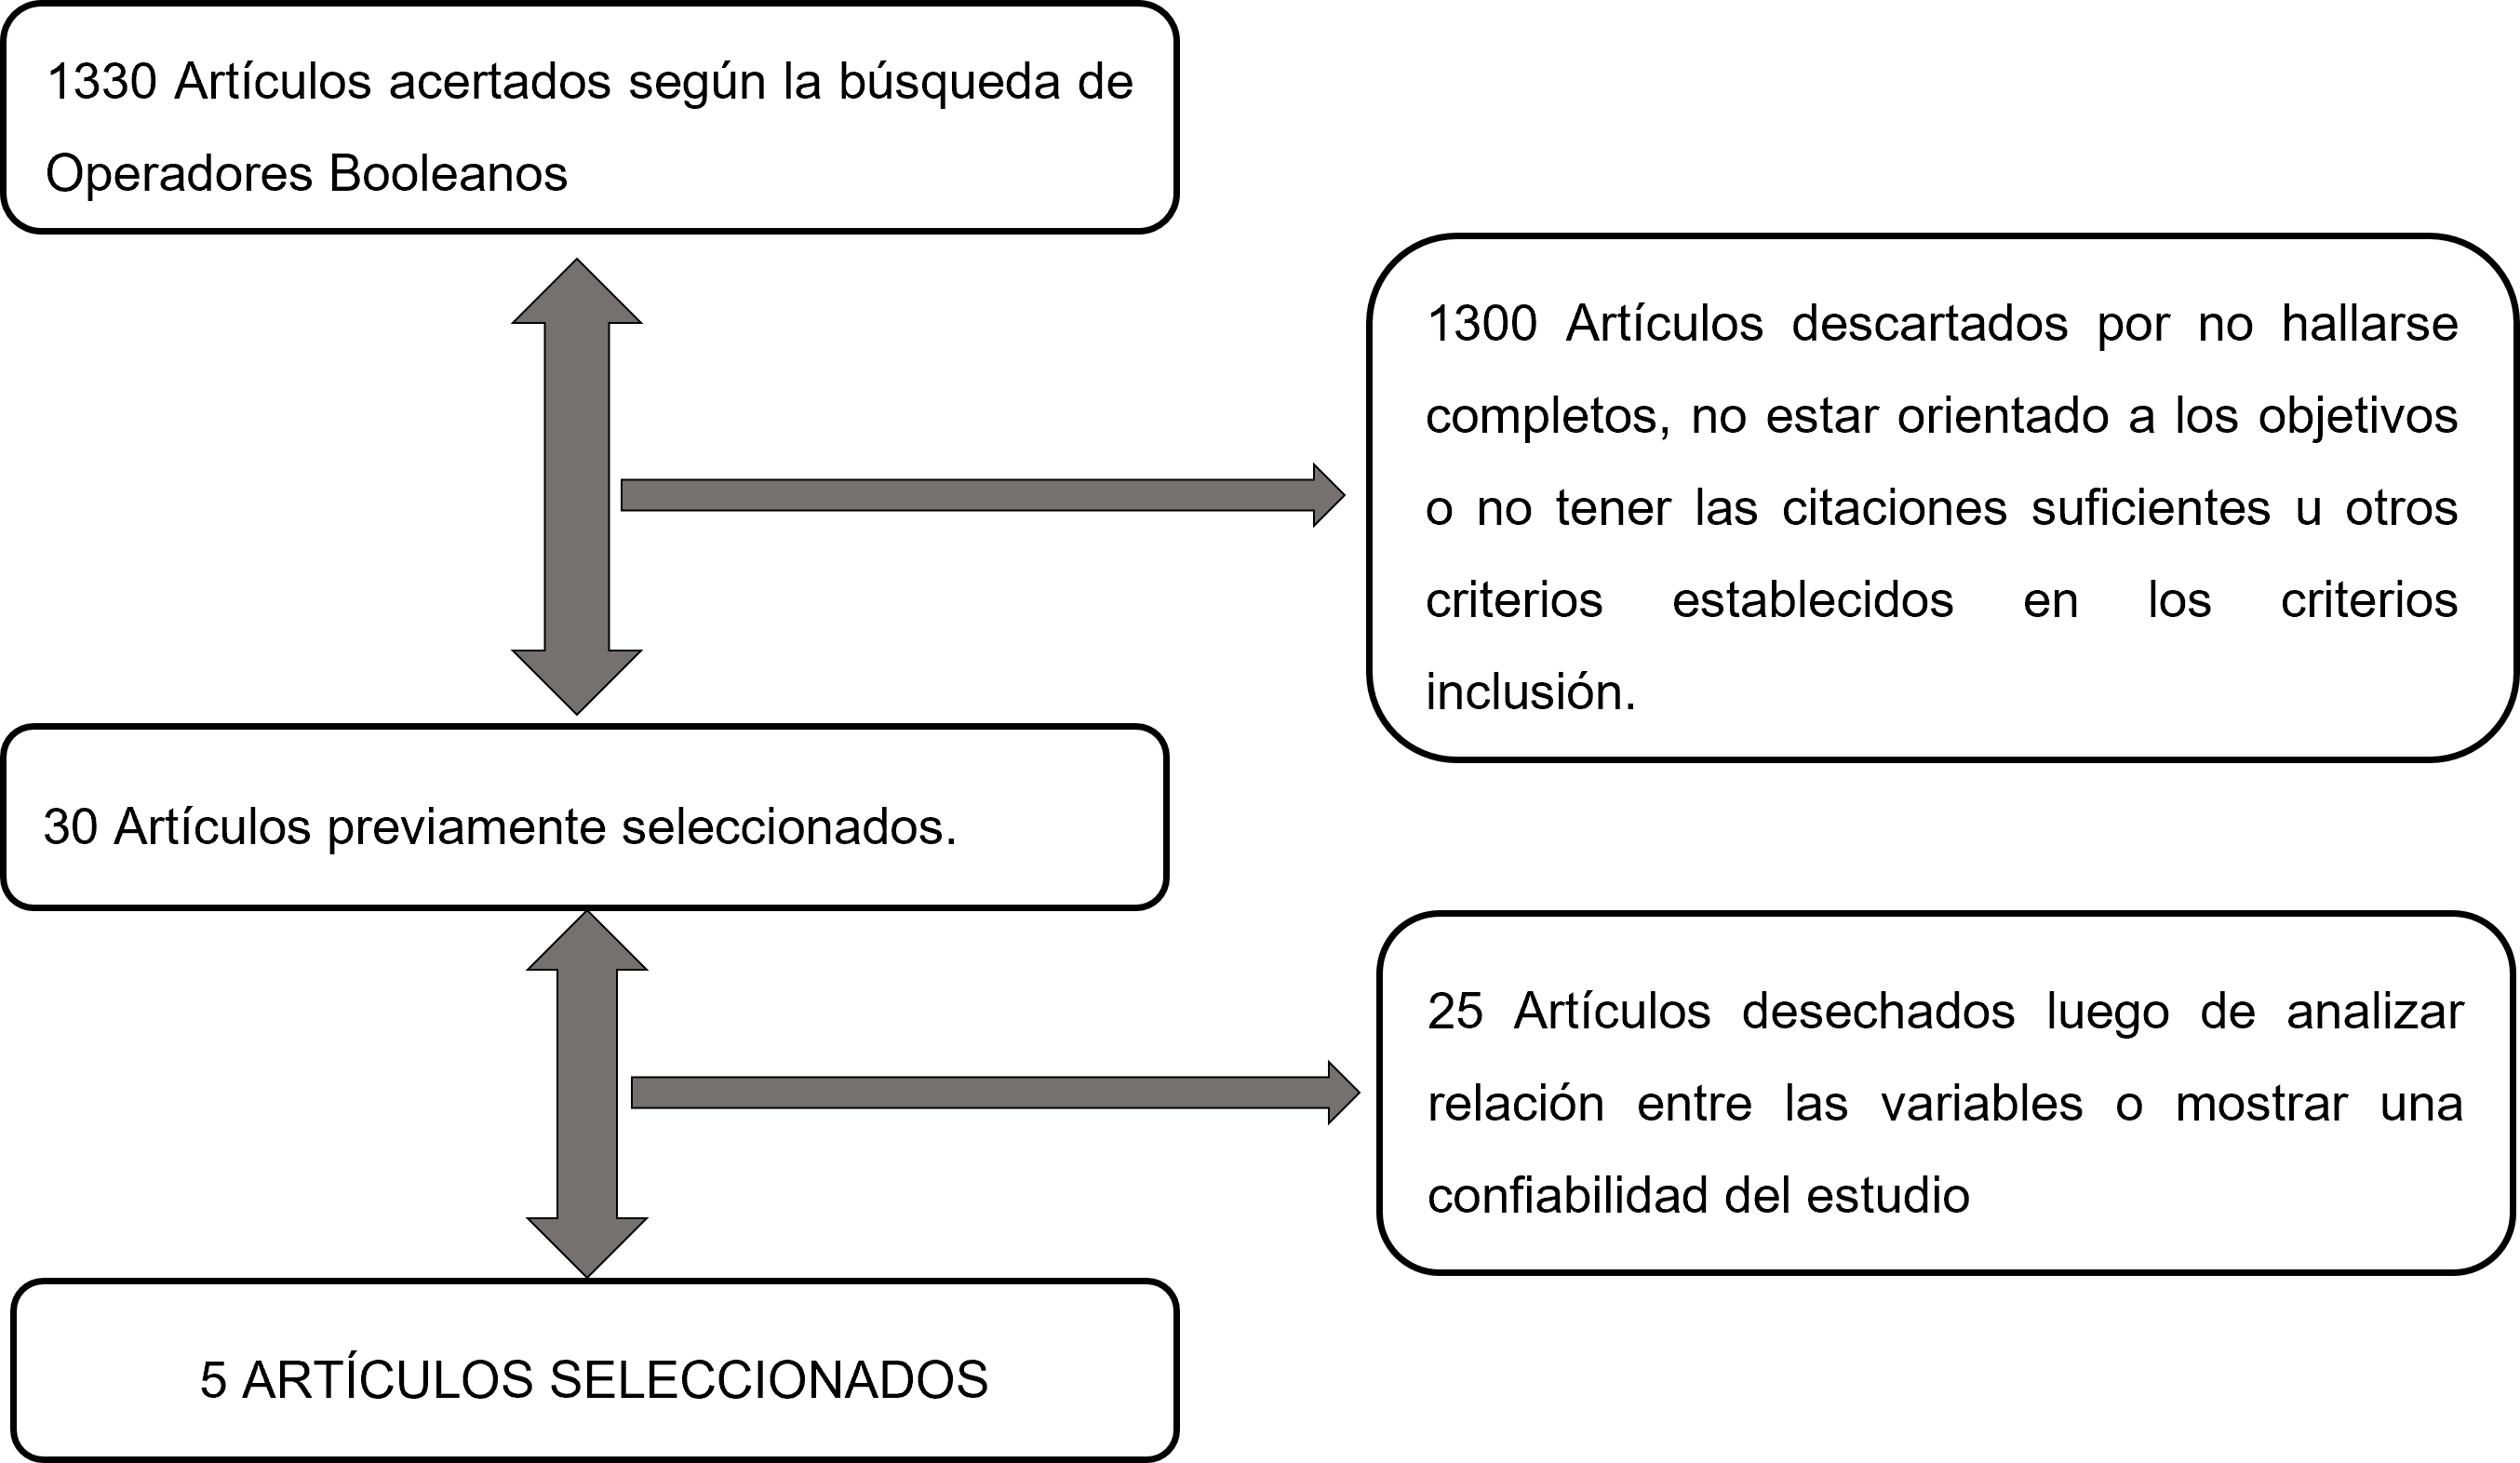
\includegraphics[width=1\columnwidth]{graficos/proceso-seleccion.png}
    		\caption{Proceso de Selección de Estudios}
    		\label{proceso}
    \end{figure}
    
\begin{table*}[hbtp]
    \centering
    \resizebox{1\textwidth}{!}{%
        \begin{tabular}{@{}ccccccc@{}}
        \toprule
        Categoría & Scopus & PubMed & IEEExplore & ACM & ScienceDirect & Total \\
        \midrule
        Comparación Algoritmos de Detección Objetos & 0 & 0 & 1 & 0 & 0 & 1 \\
        Detección + Salida de Voz & 0 & 1 & 0 & 0 & 0 & 1 \\
        Algoritmo Detección de Objetos & 0 & 0 & 0 & 0 & 0 & 0 \\
        Detección + Distancia/Orientación + Voz & 1 & 0 & 2 & 0 & 0 & 3 \\
        \textbf{TOTAL} & \textbf{1} & \textbf{1} & \textbf{3} & \textbf{0} & \textbf{0} & \textbf{5} \\
        \bottomrule
        \end{tabular}%
    }
    \caption{Resultados por categoría en diferentes bases de datos.}
    \label{seleccion-final}
\end{table*}

    \subsection{Análisis de datos}
	En el análisis de los cinco artículos seleccionados mostrados en las Tablas \ref{articulo-1}, \ref{articulo-2}, \ref{articulo-3}, \ref{articulo-4} y \ref{articulo-5} se ha evaluado una serie de criterios fundamentales para determinar su idoneidad en el contexto de la investigación sobre discapacidad visual. Los criterios abordados incluyen la adecuación de los títulos, la relevancia temporal de las publicaciones, la claridad en la exposición de los objetivos de estudio, la definición de métodos, la identificación de problemas en la línea de investigación de discapacidad visual, el logro de los objetivos de investigación, la claridad y justificación de los resultados, la coherencia en los datos, resultados y conclusiones, así como la presentación de información detallada sobre la tecnología utilizada y referencias a investigaciones previas. Este análisis proporcionará una visión integral de la calidad y la aplicabilidad de los artículos en el contexto de la investigación sobre discapacidad visual.

    \begin{table*}[hbtp]
    \centering
    \resizebox{1\textwidth}{!}{%
        \begin{tabular}{@{}p{4cm}p{10cm}@{}}
        \toprule
        \multicolumn{8}{c}{\textbf{Artículo 1}}\bottomrule \\
        Autor(es) & Samkit Shah, Jayraj Bandariya, Garima Jain, Mayur Ghevariya, Sarosh Dastoor \\
        Año & 2019 \\
        Título & ''CNN based Auto-Assistance System as a Boon for Directing Visually Impaired Person \cite{art1}'' \\
        URL & \url{https://doi.org/10.1109/ICOEI.2019.8862699} \\
        Resumen & La discapacidad visual representa un desafío significativo en la vida cotidiana de muchas personas, lo que ha llevado al desarrollo de herramientas tecnológicas innovadoras para ofrecer apoyo y autonomía. En este contexto, el artículo de investigación examina la utilidad de dos algoritmos, Haar Cascade y Convolutional Neural Network (CNN), en la detección de objetos en tiempo real, con el propósito de mejorar la vida de personas ciegas. A través de un estudio comparativo, se evaluó la precisión de ambos algoritmos utilizando una base de datos de 2300 imágenes que contenían tres clases de objetos. Para el algoritmo Haar Cascade, se utilizó un enfoque basado en características Haar-like y se entrenaron tres clasificadores diferentes. Para el algoritmo CNN, se utilizó una red neuronal convolucional pre-entrenada y se ajustaron los parámetros de aprendizaje y clasificación de imágenes. A pesar de que el algoritmo Haar Cascade demostró ser más rápido, la CNN exhibió una mayor precisión, alcanzando aproximadamente un 80\%. Este estudio destaca la eficacia de la CNN en aplicaciones de asistencia para personas con discapacidad visual, subrayando la importancia de utilizar tecnologías avanzadas para mejorar la calidad de vida de este grupo demográfico. \\
        \bottomrule
        \end{tabular}%
    }
    \caption{Información del Artículo 1.}
    \label{articulo-1}
\end{table*}

	
	\addtocontents{toc}{\protect\setcounter{tocdepth}{1}}
%%%%%%%%%%%%%%%%%%%%%%%%%%%%%%%%%%%%%%%%%%%%%%%%%%%%%%%%%%%%%%%%%%%%%%%%%%%%%%%%%%%%%%%%%%%%%%5	
	
	
	\section{Resultados}
	\subsection{Resultados de cadena redefinida}
	gfhgfh. Por se ingfhrta esta cadena de búsqueda como la definitiva.
		
	gfhfghhgghf.
	
	
	
	\section{Análisis y discusión de resultados}
	\subsection{Criterios de inclusión y exclusión}
	gfhhfgseguido por otros términos.
	\begin{table*}[hbtp]
    		\centering
    		\begin{tabular}{p{2cm} p{4cm} p{4cm} p{4cm}}
            \toprule
              Repositorio & Articulos seleccionados & Palabras detectados en todos los artículos (Titulo / Abstract) & Palabras detectados en artículos seleccionados (Titulo / Abstract) \\
            \midrule
                      ACM &                   24/50 &                                            450/473 &                                             71/234 \\
                     IEEE &                    5/50 &                                             69/450 &                                              17/51 \\
                   Scopus &                   1 / 1 &                                                 -- &                                                 -- \\
            ScienceDirect &                    4/50 &                                             70/266 &                                              15/46 \\
            \bottomrule
            \end{tabular}
    		\caption{Selección de artículos basada en análisis de titulo y abstract, detección de palabras claves en el titulo y abstract de revistas científicas.}
    		\textbf{Nota:} Los datos de Scopus no se tomaron en cuenta porque se considera menos relevantes para nuestro interés.
    		\label{seleccion_table}
    \end{table*}
    
    \begin{figure*}[hbtp]
    		\centering
    		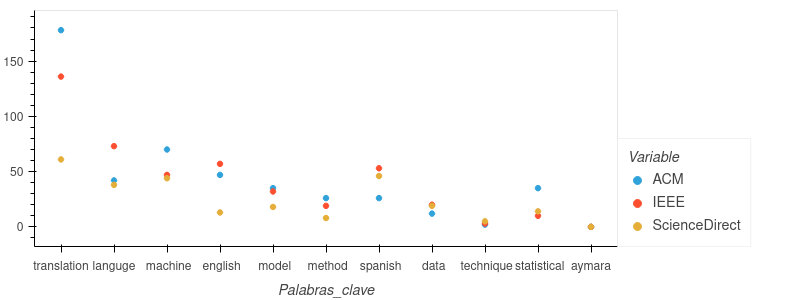
\includegraphics[width=2.3\columnwidth]{escudos/resumen_abstract..png}
    		\caption{Distribución de palabras claves en el abstract del total de revistas(50).}
    		\label{res_abs_w1}
    \end{figure*}
    \begin{figure*}[hbtp]
    		\centering
    		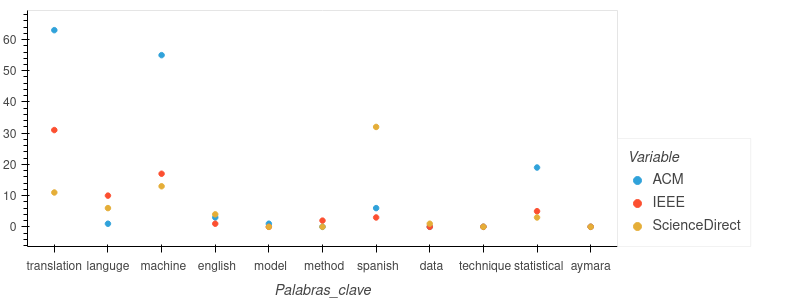
\includegraphics[width=2.3\columnwidth]{escudos/resumen_titulo.png}
    		\caption{Distribución de palabras claves en el titulo del de revistas seleccionados.}
    		\label{res_tit_w2}
    \end{figure*}
    
	\subsection{Respuestas a las preguntas }
	\begin{itemize}
	    \item ¿Existen modelos de traducción automática para traducir la lengua nativa aimara a español ?\\
	    
	    \textbf{Respuesta:}\\
	    gfhgfghfpus, que incluyen los sistemas estadísticos (SMT). Cuando se dispone de un corpus paralelo escaso, RBMT se vuelve particularmente atractivo \cite{10.1145/2738045}.\\
	    Para el pfhghf
	    
	    \textbf{Respuesta:}\\
	    Los sistemas de tgfhrte en las referencias sean lo más consistentes posible \cite{10.1109/TASLP.2020.3042006} \cite{8614221}.
	    \item ¿Que arquitectura de redes neuronales se usan para traducción automática de lenguas?\\
	    
	    \textbf{Respuesta:}\\
	    Una forma bágfhscomposición en el decodgfhar una arquitectura de red neuronal recurrente (RNN) \cite{DBLP:journals/corr/LuongPM15} \cite{DBLP:journals/corr/JeanCMB14}.
	    \item ¿Existe base de datos de traducciones de aimara a español?\\
	    
	    \textbf{Respuesta:}\\
	    Base dgfhespectivas.
	\end{itemize}
	\section{Conclusiones}
	\begin{itemize}
	    \item Lfgh pocos trabajos, pero también menos relevantes a criterio de los autores.
	    \item Traducción automática (Neural Machine translation) de la lengua aymara a español es una pgfhversa.  
	\end{itemize}
	
	\printbibliography[heading=bibintoc]
	
\end{document}